%===================================== CHAP 4 =================================

\chapter{Experimental results}

\section{Experimental setup}
\subsection{Marine Cybernetics Laboratory}
The Marine Cybernetics laboratory (MC-lab) is a small wave basin laboratory with the Department of Marine Technology at NTNU. Due to its relatively small size and advanced instrumentation package, the facility is especially suited for tests of motion control system for marine vessels, but is also suitable for more specialized hydrodynamic tests due to the advanced towing carriage, which has capability for precise movement of models up to six degrees-of-freedom for both surface ships and submersibles. The basin measures 40x6.45x1.5 meter in length, width and depth, displayed in Fig. \ref{fig:labpic}. 

\begin{figure}[!h]
    \centering
    \makebox[\textwidth][c]{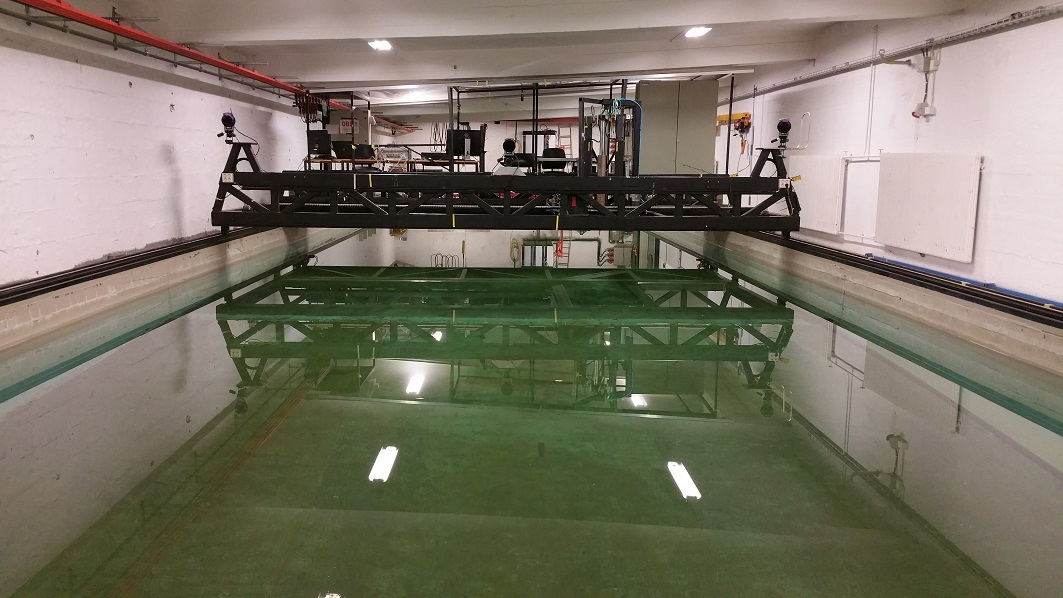
\includegraphics[width=0.7\textwidth]{fig/mclab.jpg}}
    \caption{MC-lab basin (Picture from MCLab Handbook)\cite{MClab}}
\end{figure}\label{fig:labpic}

\subsection{Hardware}

The lab is equipped with a Qualisys QTM (Qualisys Track Manager) system for motion capture and measurements, which is used for position feedback to the on-board control system of scale models. Input to the Qualisys system comes from 3 Oqus highspeed Infrared cameras, which tracks the IR reflector orbs fitted on vessel models in the basin. The Qualisys QTM system is installed on a dedicated workstation, using P2P communication with the Oqus cameras.

Experiments can be fully supervised from a control room equipped with a dedicated computer for the QTM system and TV connected to 2 high-resolution video-cameras. The block diagram of the control system can be seen in Fig. \ref{fig:Simulink_mclab}.

The internal communications in the lab is done over IP on a dedicated WLAN network, allowing wireless control of the model vessels as well as transfer of data.

The ship model is equipped with a National Instrument CompactRIO(cRIO) embedded computer system for control computation.

\subsection{Software}

To communicate with the ship, the laptops are fitted with a substantial software suite, which includes LabVIEW Full Development System, Matlab with Simulink package as well as the National Instruments Veristand complete software suite. The full list of dependency software is listed in \cite{}.

While the Qualisys system supplies position measurements, it does not compute the velocity feedback signals needed for the control implementations in this thesis. Instead, using the position measurements, the on-board computer estimates BODY-fixed velocities for control feedback with an applied derivative filter implemented in the system block, as seen in Fig. \ref{fig:Simulink_mclab}. 


\begin{figure}
    \centering
    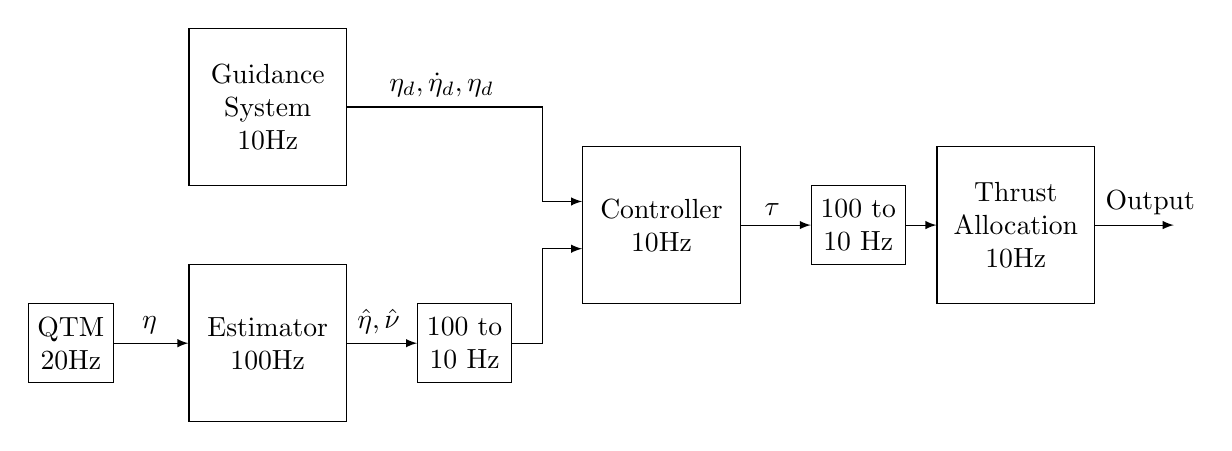
\begin{tikzpicture}
    \draw (0,0) node[minimum height=2cm,minimum width=2cm,align=center,draw] (Controller) {Controller\\ 10Hz};
    \draw (-5,1.5) node[minimum height=2cm,minimum width=2cm,align=center,draw] (Guidance) {Guidance\\ System\\ 10Hz};
    \draw (-5,-1.5) node[minimum height=2cm,minimum width=2cm,align=center,draw] (Estimator) {Estimator\\ 100Hz};
    \draw (4.5,0) node[minimum height=2cm,minimum width=2cm,align=center,draw] (Thrust) {Thrust\\ Allocation\\ 10Hz};
    \draw (-7.5,-1.5) node[minimum height=1cm,minimum width=1cm,align=center,draw] (Input1) {QTM\\ 20Hz};
    \draw (-2.5,-1.5) node[minimum height=1cm,minimum width=1cm,align=center,draw] (10HZ1) {100 to\\
    10 Hz};
    \draw (2.5,0) node[minimum height=1cm,minimum width=1cm,align=center,draw] (10HZ2) {100 to\\
    10 Hz};
    
    \draw[-latex] (Input1.east) -|([xshift=0.45cm] Input1.east) node[above]{$\eta$} |- (Estimator.west);
    
    \draw[-latex] (Estimator.east) -| ([xshift=0.4cm] Estimator.east) node[above]{$\hat{\eta},\hat{\nu}$} |- (10HZ1.west);
    
    
    \draw[-latex] (10HZ1.east) -| ([xshift=-0.5cm,yshift=-0.3cm] Controller.west)  |- ([yshift=-0.3cm]Controller.west);
    
    
    \draw[-latex] (Guidance.east) -|([xshift=1.2cm] Guidance.east) node[above]{$\eta_d, \dot{\eta}_d, \Ddot{\eta}_d$} -| ([xshift=-0.5cm,yshift=0.3cm] Controller.west) |- ([yshift=0.3cm] Controller.west);
    
    \draw[-latex] (Controller.east) -| ([xshift=0.4cm] Controller.east) node[above]{$\tau$} |- (10HZ2.west);
    
    \draw[-latex] (Thrust.east) -| ([xshift=0.7cm] Thrust.east) node[above]{Output} |- ([xshift=1cm] Thrust.east);
    
    \draw[-latex] (10HZ2.east) |- (Thrust.west);

    \end{tikzpicture}
    \caption{MC-Lab Simulink setup}
    \label{fig:Simulink_mclab}
\end{figure}

\section{Lab session 1 - March}
In this section, surface plots of the model ship will be presented. For visibility, the length of the CSAD model has been scaled by 1:6, from the original 2.578m, since the 4-corner test maneuvers within a 4x4 square in the lab basin. 
To have a basis of comparison for the adaptive techniques in the laboratory experiments, an initial 4-corner test of the CSAD is done with the nonlinear pose and velocity feedback controller (NP-NV) as described in Chapter 2. The 4-corner for NP-NV test is shown in Fig.  \ref{NPNV4corner}. 

\begin{figure}[!h]
    \centering
    \makebox[\textwidth][c]{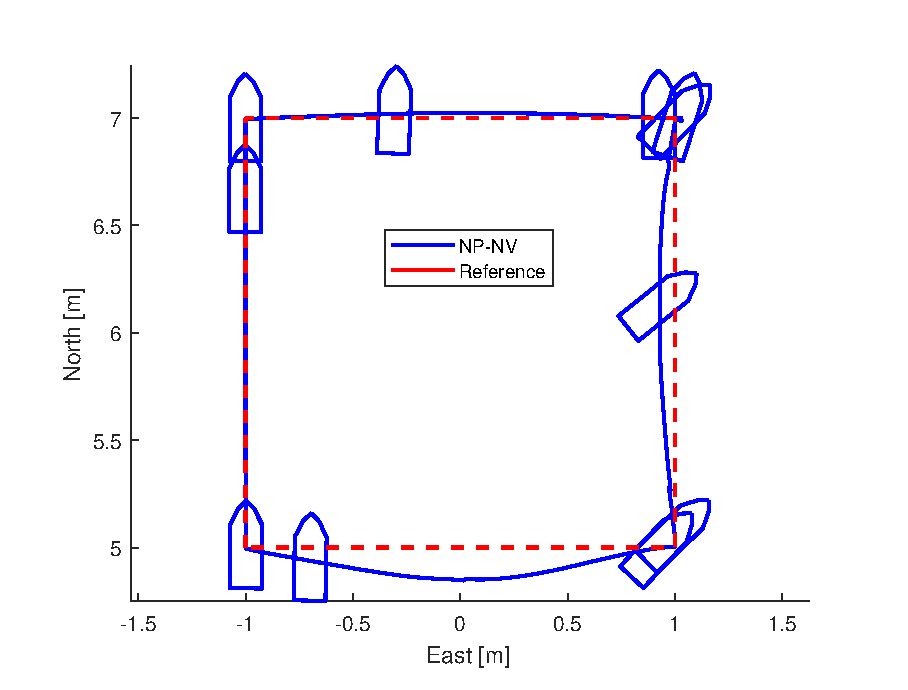
\includegraphics[width=0.7\textwidth]{plotslab1/NPNVpath}}
    \caption{Unconstrained NPNV 4-corner test. }
\end{figure}\label{NPNV4corner}



\begin{table}[h!]
\centering
\caption{Control gains}\label{table:gains1}
\begin{tabular}{|l |c|r|}
\toprule
& \textbf{$\mathcal{L}_1$}  \\
\midrule
\hline
$\boldsymbol{\Gamma}_1$ & $\text{diag}([0.08,0.08,0.0698])$  \\

$\boldsymbol{\Gamma}_2$  & $\text{diag}([0.2,0.2,0.1745])\boldsymbol{M}$   \\

$\Delta_{\tilde{p}}$  & $0.5$    \\
$\Delta_{\tilde{\psi}}$  & $0.5$    \\

$\Delta_{\tilde{v}}$  & $0.7$ \\
$\Delta_{\tilde{r}}$  & $1$ \\
$\boldsymbol{L_1}$  & $I*(2*\pi)^2$ \\
$\boldsymbol{L_2}$  & $I*2*1.2*2*\pi$ \\
$\boldsymbol{\gamma}_w_{\delta}$  & $(20*\pi)^2/4$ \\\hline
\bottomrule
\todo{Add II gain values}
\end{tabular}
\end{table}
Table \ref{table:gains1} displays the control and parameter gains used in Lab session 1. 
\subsection{$\mathcal{L}_1$ Adaptive control}

\begin{align}
    \boldsymbol{\tau} &= \boldsymbol{M}\dot{\alpha} + (\boldsymbol{C + D})\alpha - \boldsymbol{K}_2\boldsymbol{z}_2 -\boldsymbol{\hat{w_{\delta}}}  \\
    \boldsymbol{\dot{\hat{w_{\delta}}}} &=-\gamma_{w_\delta}\boldsymbol{R}\tilde{\boldsymbol{\nu}} 
\end{align}






\begin{figure}[!h]
    \centering
    \makebox[\textwidth][c]{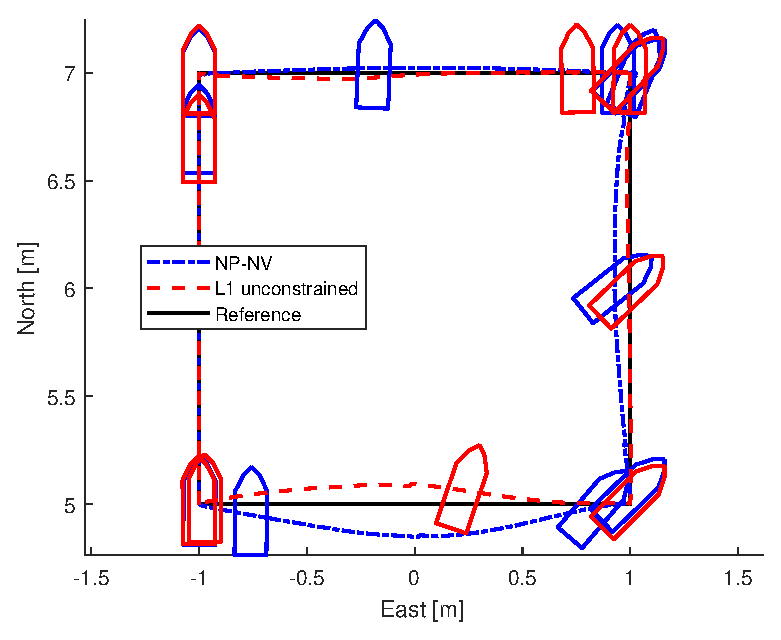
\includegraphics[width=0.8\textwidth]{plotslab1/L1path.eps}}
    \caption{Unconstrained $\mathcal{L}_1$ 4-corner test. }
\end{figure}\label{fig:L14corner}

Fig. \ref{fig:L14corner} shows the path plot of the unconstrained $\mathcal{L}_1$ cascaded controller. It can be seen that the controller follows the reference path better than the nominal NP-NV, especially for the ($4 \xrightarrow{} 4$) backwards motion in Fig. \ref{fig:4corner} where it almost keeps the pose perfectly. This is most likely due to the adaptation compensating for uncertainties in the model during motion while keeping the heading at 45$^o$.


\begin{figure}[!h]
    \centering
    \makebox[\textwidth][c]{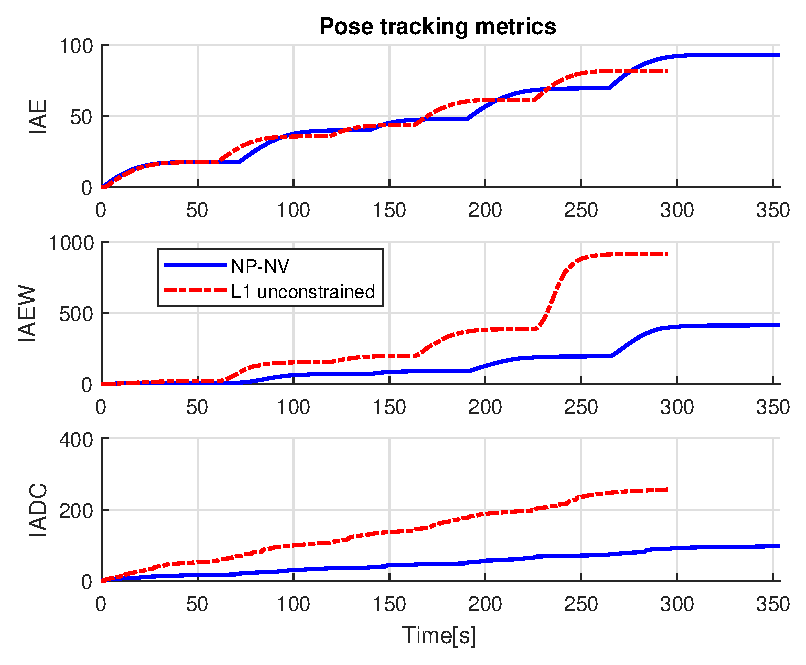
\includegraphics[width=0.8\textwidth]{plotslab1/L1metric.eps}}
    \caption{Unconstrained $\mathcal{L}_1$, Pose error metrics. }
\end{figure}\label{fig:L1unconstrMetrics}

The evolution of the performance metrics for pose error is shown in Fig. \ref{fig:L1unconstrMetrics}. One can see that the $\mathcal{L}_1$ controller performs the 4 corner faster than the NP-NV, and with lower pose error(IAE). However, the energy consumption is significantly higher, due to the aggressive nature of the adaptive scheme. This is especially significant for the coupled motion in ($5 \xrightarrow{} 1$), where the controller seeks to reduce control error in both sway and yaw, simultaneously.

\begin{figure}[!h]
    \centering
    \makebox[\textwidth][c]{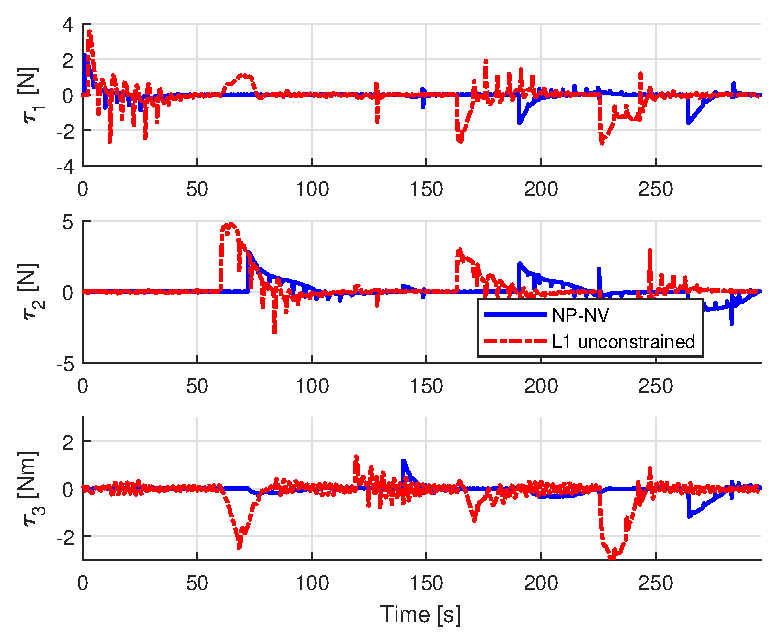
\includegraphics[width=0.8\textwidth]{plotslab1/L1tau.eps}}
    \caption{Unconstrained $\mathcal{L}_1$, Control input. }
\end{figure}\label{fig:L1unconstTau}

Fig. \ref{fig:L1unconstTau} displays the commanded control input in all degrees of freedom. There are significant spikes in the control input for the $\mathcal{L}_1$, which can be attributed not only to the aggressive adaptation, but also to the fact that the adaptation is more susceptible to errors in the measurements due to the high-gain state predictor. This will be discussed further later in this chapter. 


\begin{figure}[!h]
    \centering
    \makebox[\textwidth][c]{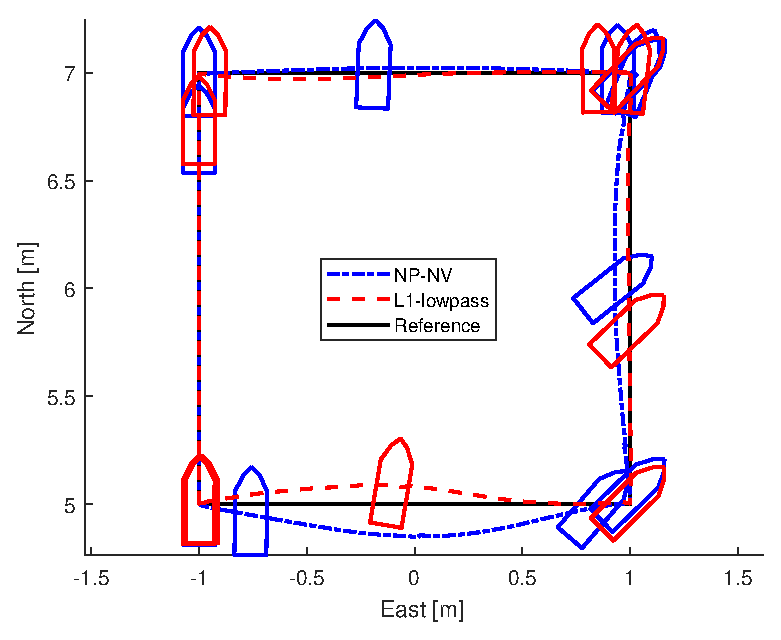
\includegraphics[width=0.8\textwidth]{plotslab1/L1LPpath.eps}}
    \caption{Lowpass filtered $\mathcal{L}_1$ 4-corner test. }
\end{figure}\label{fig:L1LP4corner}

In Fig. \ref{fig:L1LP4corner}, the $\mathcal{L}_1$ has been run with a Low-pass filter fitted to the control input, cut-off frequency at 100 Hz. The desired goal was to reduce noice in the commanded input to the ship. The path plot, as well as the IAE shows that the LP did not reduce path tracking.  Unfortunately, this did not have much effect, as the noise in the control signal seen in Fig. \ref{fig:L1LPtau} is most likely within the cut-off. 

\begin{figure}[!h]
    \centering
    \makebox[\textwidth][c]{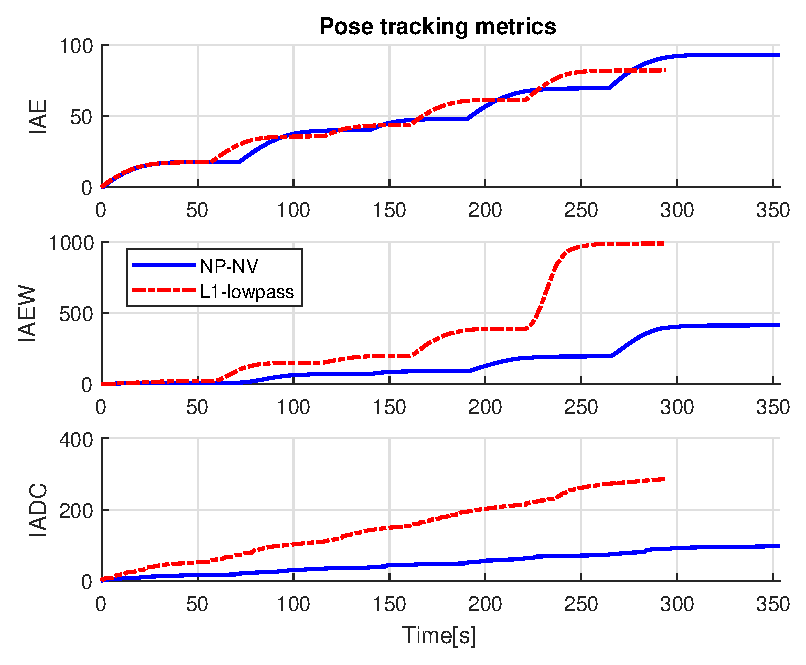
\includegraphics[width=0.8\textwidth]{plotslab1/L1LPmetric.eps}}
    \caption{Lowpass filtered $\mathcal{L}_1$ , Pose error metrics. }
\end{figure}\label{fig:L1LPMetrics}


\begin{figure}[!h]
    \centering
    \makebox[\textwidth][c]{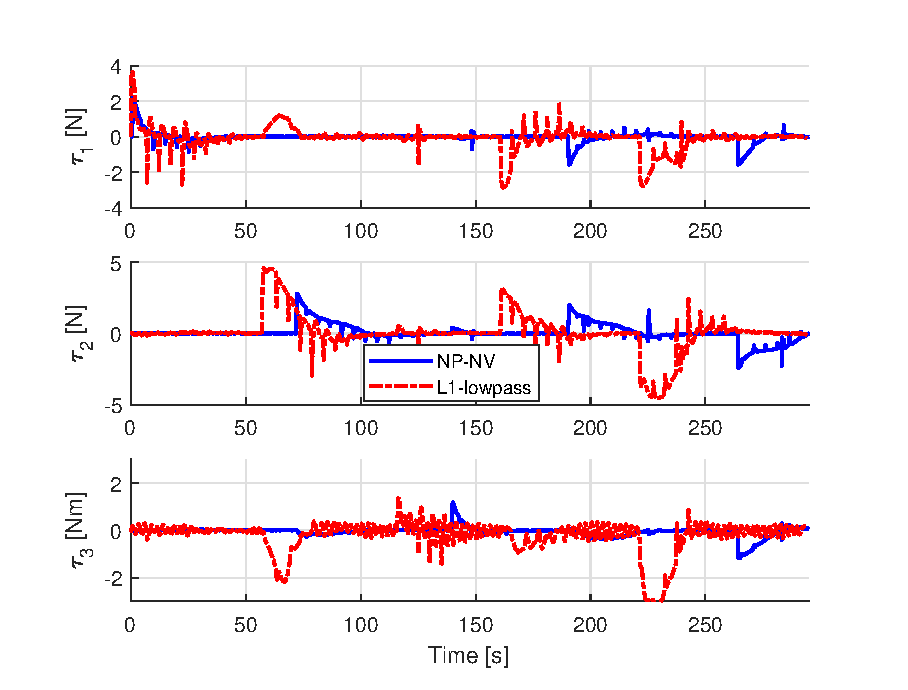
\includegraphics[width=0.8\textwidth]{plotslab1/L1LPtau.eps}}
    \caption{Lowpass filtered $\mathcal{L}_1$, Control input. }
\end{figure}\label{fig:L1LPtau}


\begin{figure}[!h]
    \centering
    \makebox[\textwidth][c]{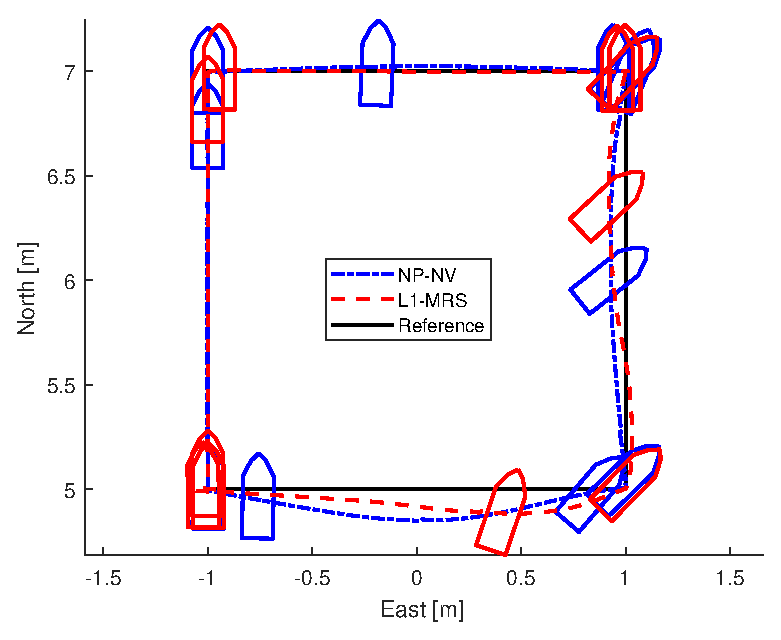
\includegraphics[width=0.8\textwidth]{plotslab1/L1MRS1path.eps}}
    \caption{ $\mathcal{L}_1$ with MRS 4-corner test. Rate constraints are increased by 1.2. }
\end{figure}\label{fig:L1MRS14corner}

Fig. \ref{fig:L1MRS14corner} shows the path of the $\mathcal{L}_1$ controller enhanced with an MRS-model to limit the control input to the ship. Initially, the $\mathcal{L}_1$-MRS was run with the rate constrains in Table \ref{}, but it resulted in significant overshoot, likely due to the rate limits being to conservative for the aggressive controller. In this test, the limits are increased by a factor of 1.2. The ship follows the reference better than the nominal NP-NV, but not as good as the unconstrained $\mathcal{L}_1$. This could be due to too strict limits on both the magnitude and rate of the MRS model. 

\begin{figure}[!h]
    \centering
    \makebox[\textwidth][c]{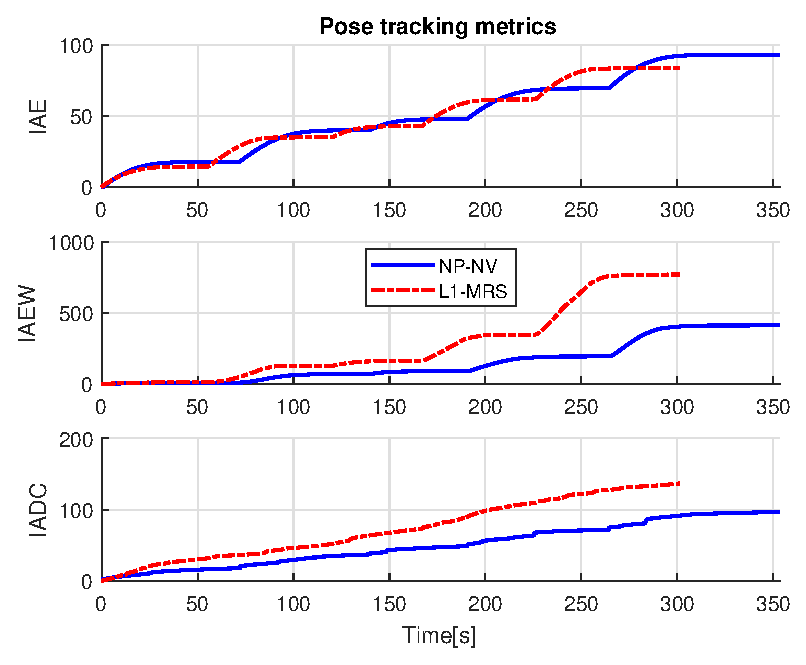
\includegraphics[width=0.8\textwidth]{plotslab1/L1MRS1metric.eps}}
    \caption{ $\mathcal{L}_1$ with MRS, Pose error metrics. Rate constraints are increased by 1.2. }
\end{figure}\label{fig:L1MRS1Metrics}

In Fig. \ref{fig:L1MRS1Metrics}, the evolution of the metrics is shown. As with the unconstrained test of $\mathcal{L}_1$, the MRS-fitted controller is faster to complete the 4-corner test than the nominal, but with higher IAEW and IADC. Nonetheless, it can be noted that the MRS reduces the energy consumption by the IAEW in comparison to the unconstrained $\mathcal{L}_1$, as seen in Table \ref{performancemetrics1}. 

\begin{figure}[!h]
    \centering
    \makebox[\textwidth][c]{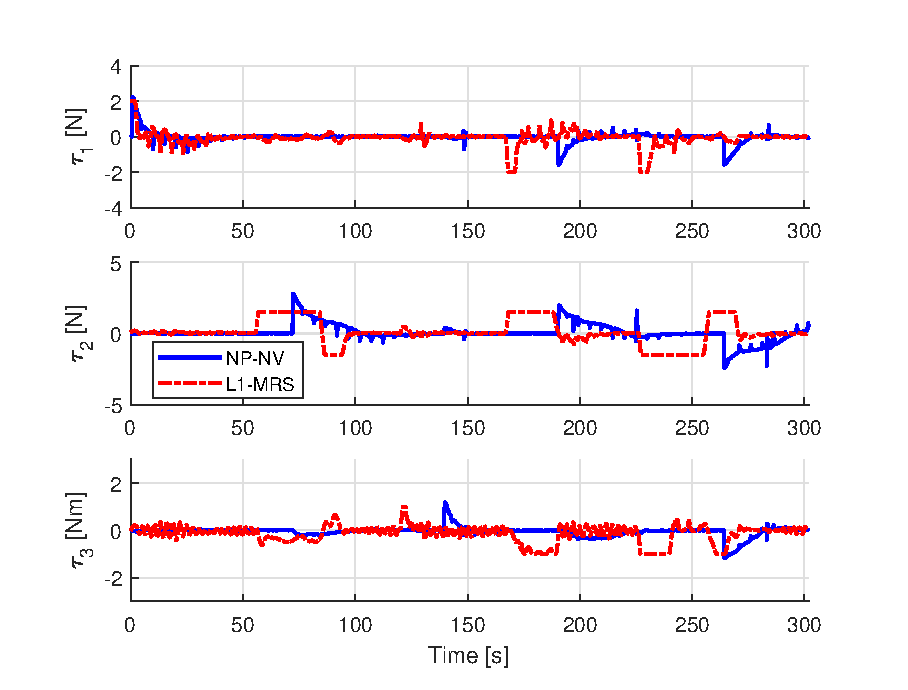
\includegraphics[width=0.8\textwidth]{plotslab1/L1MRS1tau.eps}}
    \caption{ $\mathcal{L}_1$with MRS, Control input. Rate constraints are increased by 1.2. }
\end{figure}\label{fig:L1MRS1tau}

The effects of the magnitude limits of the MRS is seen in Fig. \ref{fig:L1MRS1tau}, where especially the commanded force in sway is limited, and lower than the nominal.

\begin{figure}[!h]
    \centering
    \makebox[\textwidth][c]{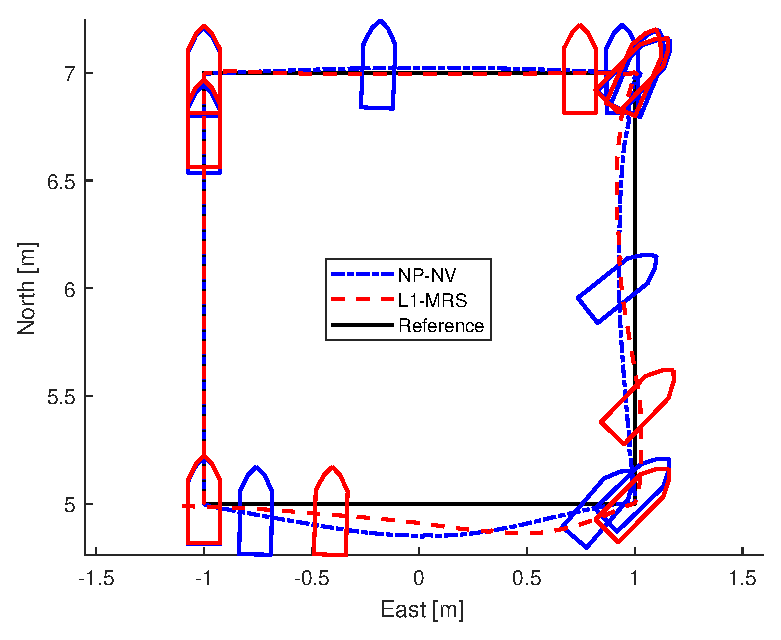
\includegraphics[width=0.8\textwidth]{plotslab1/L1MRS2path.eps}}
    \caption{ $\mathcal{L}_1$ with MRS 4-corner test. Rate constraints are increased by 1.5. }
\end{figure}\label{fig:L1MRS24corner}

Since the results from the first $\mathcal{L}_1$-MRS test could indicate that the saturation limits were not liberal enough, a new experiment was done with increasing the rate limits with a factor of 1.5. The path plot for this experiment is shown in Fig. \ref{fig:L1MRS24corner}. Unfortunately, this did not lead to better tracking, as the path and the IAE are similar to the MRS test with rate factored by 1.2. This indicates that the perhaps the issue is not only with the rate but also with the magnitude limitations set. 

\begin{figure}[!h]
    \centering
    \makebox[\textwidth][c]{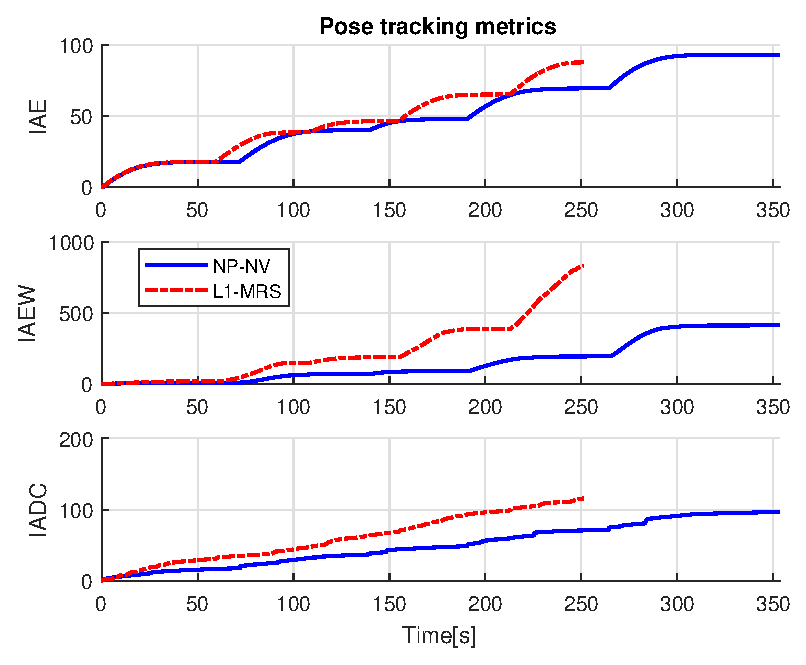
\includegraphics[width=0.8\textwidth]{plotslab1/L1MRS2metric.eps}}
    \caption{ $\mathcal{L}_1$ with MRS, Pose error metrics. Rate constraints are increased by 1.5. }
\end{figure}\label{fig:L1MRS2Metrics}

Even though the increased rate limitations of the MRS fitted on $\mathcal{L}_1$ does not improve tracking, the wear on actuators, by the IADC metric were reduced by the more liberal rate limit, a reduction of approximately 11 percent , as seen in Table \ref{performancemetrics1}.

\begin{figure}[!h]
    \centering
    \makebox[\textwidth][c]{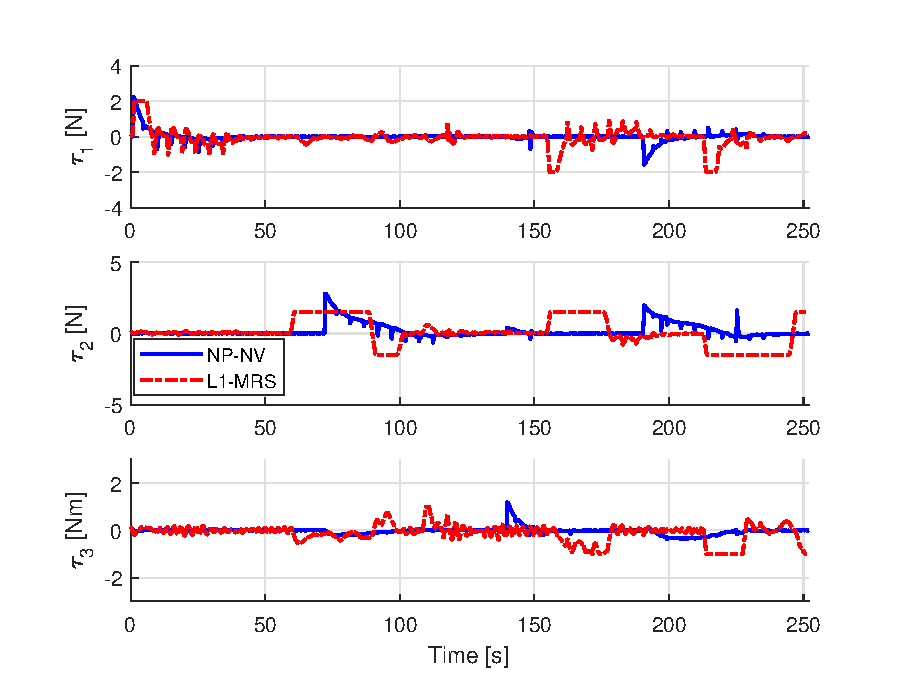
\includegraphics[width=0.8\textwidth]{plotslab1/L1MRS2tau.eps}}
    \caption{ $\mathcal{L}_1$with MRS, Control input. Rate constraints are increased by 1.5. }
\end{figure}\label{fig:L1MRS2tau}

\newpage
\subsection{Immersion and Invariance adaptive control}

\begin{align}
    \boldsymbol{\tau} &= \\
    \boldsymbol{\dot{\hat{\sigma}}} &= 
\end{align}
\todo{Add control and adaptation law}

\begin{figure}[!h]
    \centering
    \makebox[\textwidth][c]{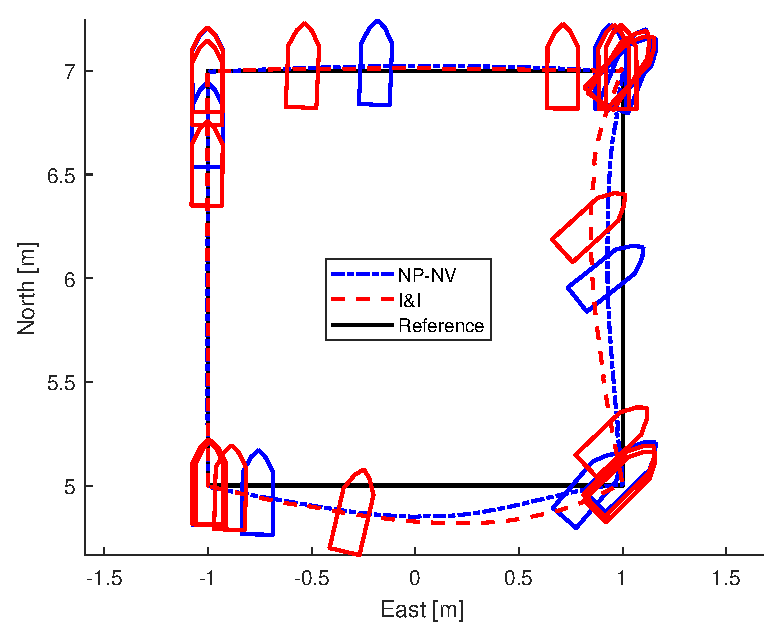
\includegraphics[width=0.8\textwidth]{plotslab1/IIpath.eps}}
    \caption{Unconstrained I\&I 4-corner test. }
\end{figure}\label{fig:II4corner}

The 4-corner path of the I\&I adaptation is shown in Fig. \ref{fig:II4corner}. As with the $\mathcal{L}_1$ adaptive, the I\&I is adaptation fitted to the nominal NP-NV cascaded nonlinear feedback controller. Although, in this case the adaptation seems to deteriorate the reference tracking ability, as seen in the pose error metrics in Fig. \ref{fig:IImetric}.

\begin{figure}[!h]
    \centering
    \makebox[\textwidth][c]{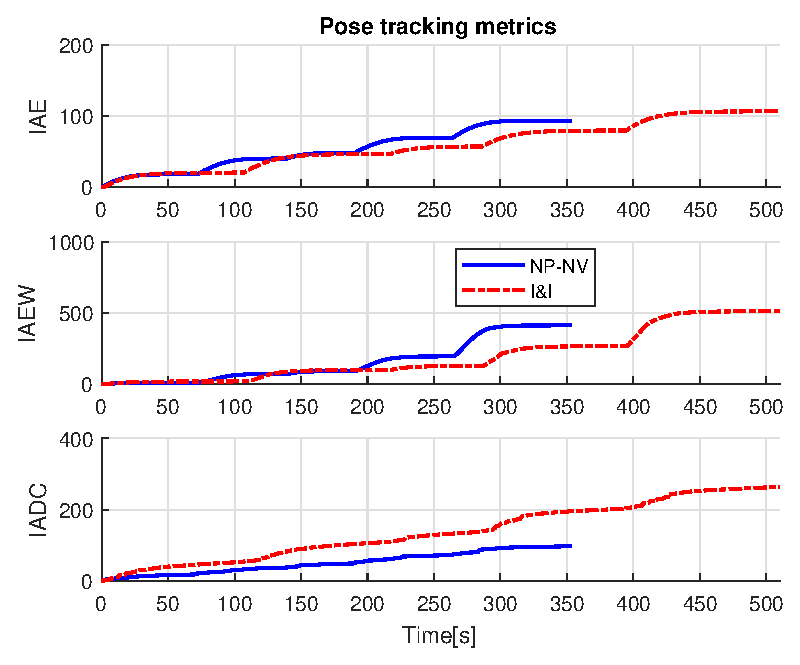
\includegraphics[width=0.8\textwidth]{plotslab1/IImetric.eps}}
    \caption{Unconstrained I\&I , Pose error metrics.}
\end{figure}\label{fig:IImetric}

Additionally, the adaptation also appears to slow the controller down by almost 150 seconds overall on the 4-corner maneuver. This could suggest that the tuning of the adaptive parameter gains are not sufficiently accurate, causing the adaptation to not compensate for the inherent uncertainties in the model, but on the contrary worsen the performance. Moreover, as seen in Fig. \ref{fig:IItau}, similarly to $\mathcal{L}_1$ , the I\&I adaptation is more susceptible to noise in the feedback signals.  

\begin{figure}[!h]
    \centering
    \makebox[\textwidth][c]{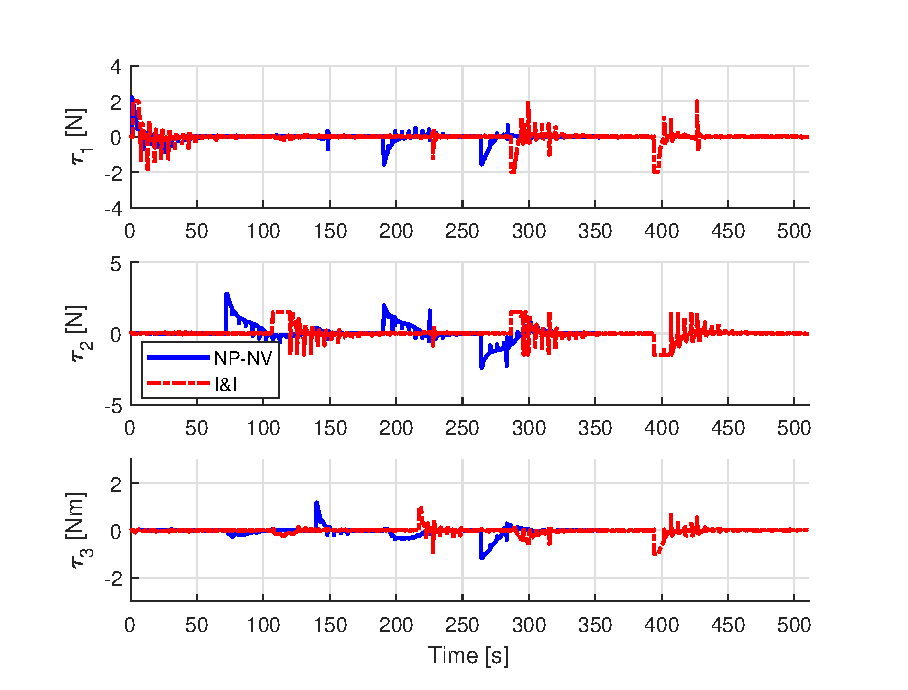
\includegraphics[width=0.8\textwidth]{plotslab1/IItau.eps}}
    \caption{Unconstrained I\&I , Control input.}
\end{figure}\label{fig:IItau}

\begin{figure}[!h]
    \centering
    \makebox[\textwidth][c]{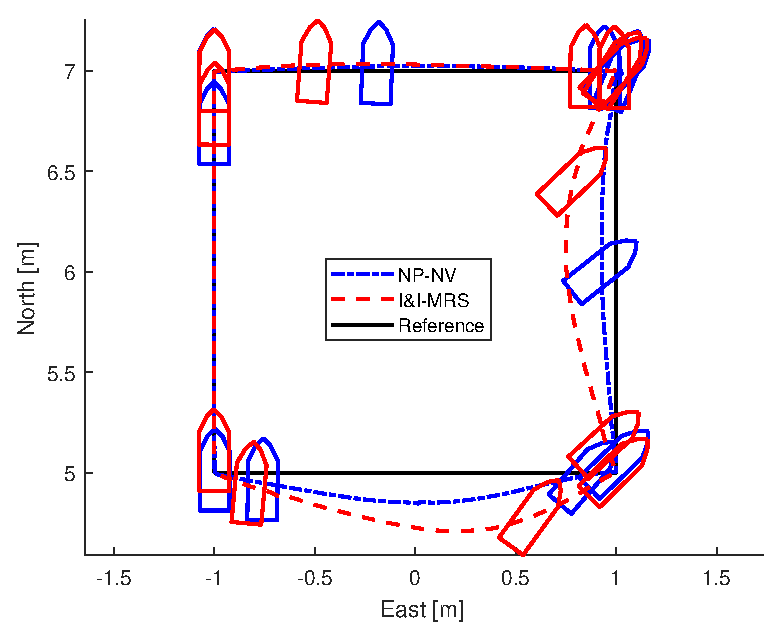
\includegraphics[width=0.8\textwidth]{plotslab1/IIMRSpath.eps}}
    \caption{I\&I with MRS, 4-corner test. }
\end{figure}\label{fig:IIMRS4corner}

The I\&I is then tested with the MRS model fitted, using the rate limits from Table \ref{table}, to which the path plot is shown in Fig. \ref{fig:IIMRS4corner}. Even though it might look as the performance is worsened compared to the unconstrained test, the MRS limited I\&I achieved the same overall pose error, as seen in Fig. \ref{fig:IIMRSmetric} and Table \ref{performancemetrics1}. Moreover, the IADC metric illustrating actuator wear is lowered compared to the nominal NP-NV. This is reasonably assumed to be due to the limiting effects of the MRS-model. 

\begin{figure}[!h]
    \centering
    \makebox[\textwidth][c]{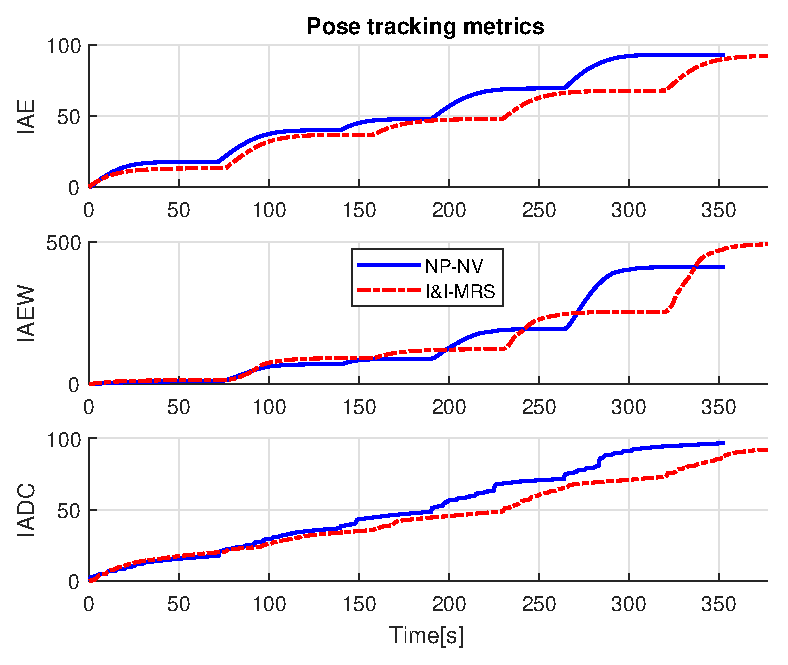
\includegraphics[width=0.8\textwidth]{plotslab1/IIMRSmetric.eps}}
    \caption{I\&I with MRS , Pose error metrics.}
\end{figure}\label{fig:IIMRSmetric}

As the metrics in Fig .\ref{fig:IImetric} show, the I\&I-MRS control system still has higher energy consumption than NP-NV.

\begin{figure}[!h]
    \centering
    \makebox[\textwidth][c]{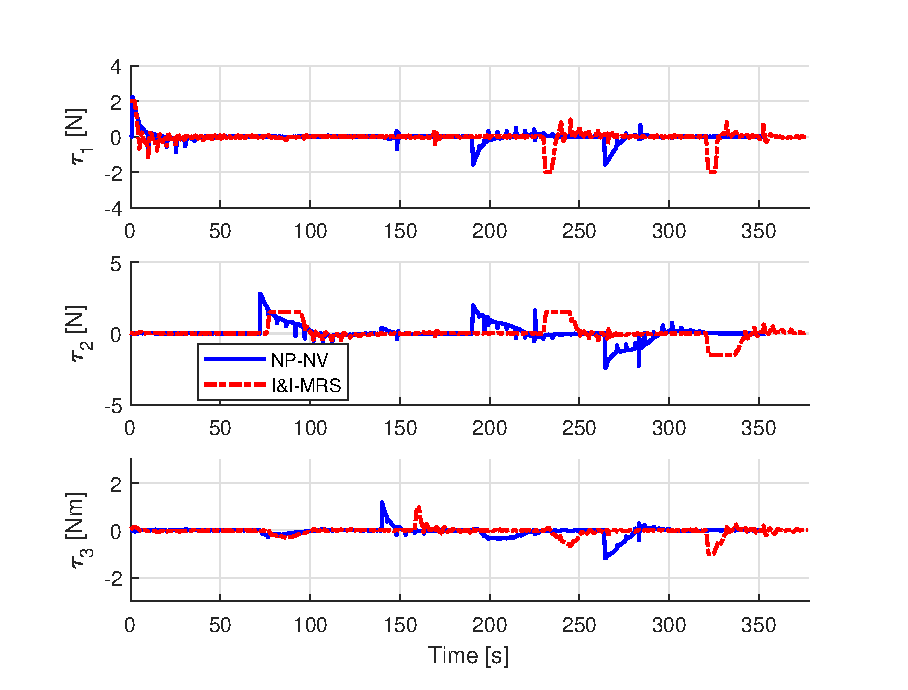
\includegraphics[width=0.8\textwidth]{plotslab1/IIMRStau.eps}}
    \caption{I\&I with MRS , Control input.}
\end{figure}\label{fig:IIMRStau}

\subsection{Summary of lab session 1}

 Concluding the experiments from the first lab session, there are some key findings to note; When evaluating the controllers overall ability to reduce control error during the 4-corner test, the unconstrained $\mathcal{L}_1$ adaptive scheme is the most capable in terms of the IAE metric, especially in the ($4 \xrightarrow{} 4$) backwards motion as seen in Fig. \ref{fig:4corner}. For this motion, all other controllers seem to relax the keeping of the East coordinate, as well as several degrees in heading keeping, while $\mathcal{L}_1$ manages to keep the East and heading at a small error. Admittedly, the aggressiveness of the $\mathcal{L}_1$ does lead to a higher energy consumption and actuator wear. The experiments with using an MRS model in cascade with $\mathcal{L}_1$ does seem promising in reducing these downsides, at a minimal cost to pose error, and as such this cascaded control system will be continued in the second lab session, discussed later in this chapter. Since the I\&I experiments are not as promising, the main focus will be on the $\mathcal{L}_1$ further-on. 

\todo{Maybe put a plot of yawtilde for the 4-5 motion?}
\begin{table}[h!]
\centering 
\begin{tabular}{| p{2cm} | p{2cm} | p{3cm} | p{2cm}|}
\hline
\textbf{Controller}& \textbf{IAE} &  \textbf{IAEW} &\textbf{IADC}   \\ \hline\hline
$NP-NV$ & $93$ & $410$ & $96$  \\ \hline
$\mathcal{L}_1 unconstr.$ & $81$ & $915$ & $256$  \\ \hline
$\mathcal{L}_1 LP$ & $81$ & $982$ & $282$  \\ \hline
$\mathcal{L}_1 MRS 1.2$ & $83$ & $762$ & $130$  \\ \hline
$\mathcal{L}_1 MRS 1.5$ & $85$ & $831$ & $115$  \\ \hline
$I\&I unconstr. $ & $106$ & $509$ & $261$  \\ \hline
$I\&I MRS. $ & $92$ & $490$ & $92$  \\ \hline
\end{tabular}
\caption{End values of performance metrics - pose error}
\label{performancemetrics1}
\end{table}
\todo{Bold the best/lowest values maybe?}
In Table \ref{performancemetrics1}, all the final maximum values for the tested control implementations are displayed. The metric values are rounded to the nearest integer for readability.
   

\section{Findings and Improvements}

\subsection{Velocity estimation}
When evaluating the experimental data from the first lab session, it became clear that there were some problems with the positioning camera system. During a experiment, due to a combination of calibration inaccuracies and motion, the infrared reflector orbs on the ship can cause "reflection shadow", thus leading to a small jump in position. This phenomenon is shown in Fig. \ref{fig:measurements_spring}. While the might only be 2 cm in magnitude, it occurs in a single time sample of 10 milliseconds, which results in a sudden velocity change of 2 m/s, which is not only a physically unreachable velocity for the ship, but also beyond the feasible acceleration. Since the estimated velocity is fed back into the control system, it causes the controller to try to compensate for the non-physical behavior, leading to a noisy control signal and also higher wear on the actuators.   


\begin{figure}[!h]
    \centering
    \makebox[\textwidth][c]{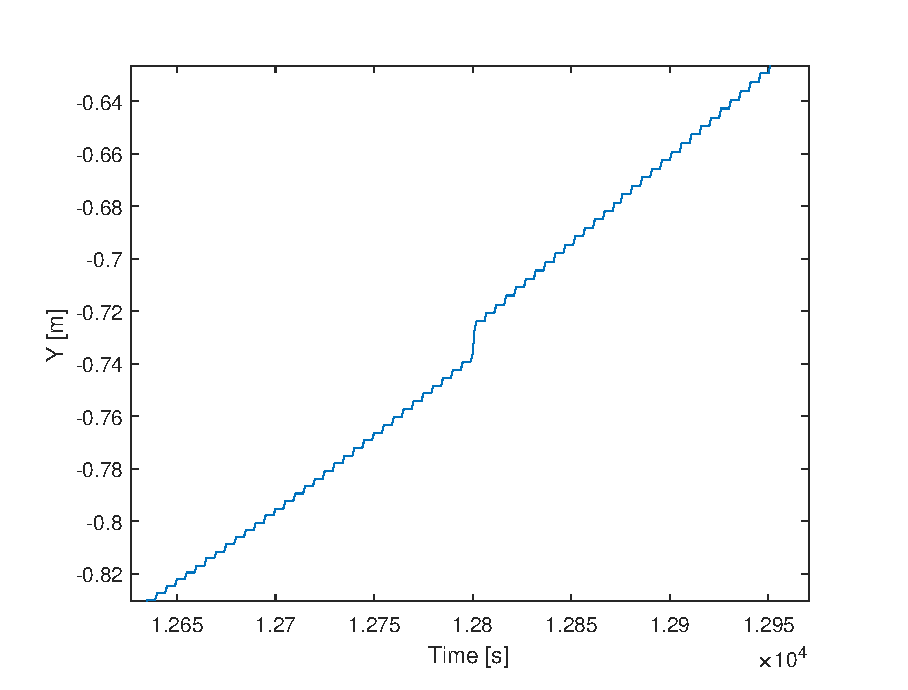
\includegraphics[width=0.7\textwidth]{plots/spring_phenomenon.eps}}
    \caption{ Jump-phenomenon in pose measurement}\label{fig:measurements_spring}
\end{figure}

The correct for this behavior, some changes to the estimator are done; 
The velocity estimator previously implemented in CSAD for the lab is a applied derivative filter. Augmenting this filter to compensate for the "spring"-effect, maximal values for CSAD feasible acceleration were set as follows: 
\begin{align}
    a_{surge}^{MAX} &= \pm 0.13 m/s^2 \\
    a_{sway}^{MAX} &= \pm 0.0267 m/s^2 \\
    a_{yaw}^{MAX} &= 0.0052 rad/s^2
\end{align}

These maximal values are determined through velocity test in the MC-lab basin, using CSAD on maximum thrust in each degree-of-freedom. Since the control system runs at 100Hz, these limit parameters are then scaled by 100 to get allowed change-per-sample, and then implemented in block form in the derivative filter. Only minor tuning is then needed to achieve optimal cutting of impulse transients in the estimated velocity signal. The final limit values are displayed in Table \ref{acc_limits_CSAD}. It should be noted that these are vessel-specific, and should be adjusted in the event of a new actuator setup, or if using the control system on another vessel. 

\begin{figure}[!h]
    \centering
    \makebox[\textwidth][c]{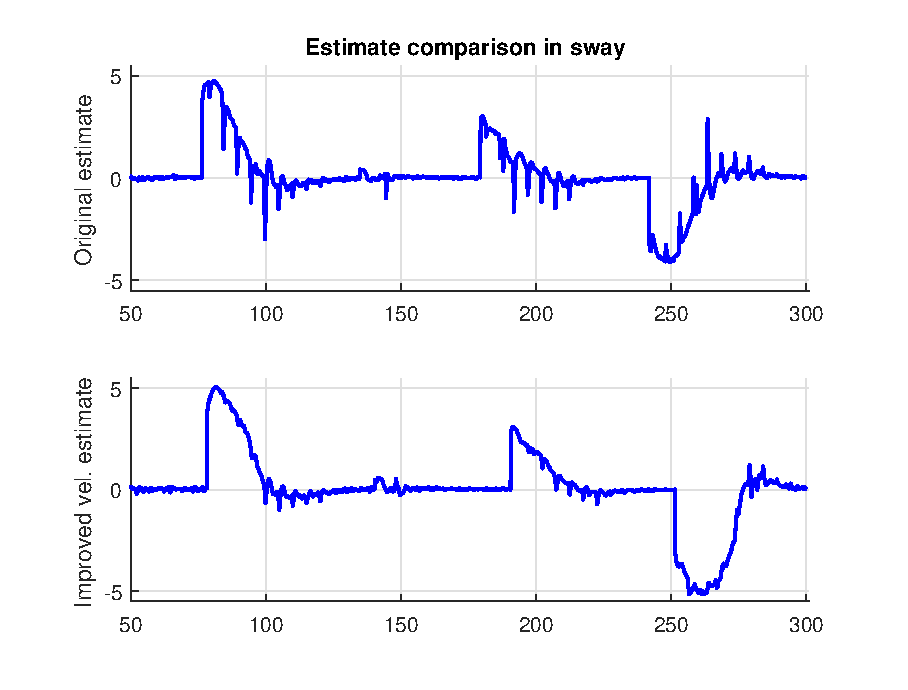
\includegraphics[width=0.85\textwidth]{plots/estimate_comparison.eps}}
    \caption{ Comparison of control input in sway with new velocity estimator}\label{fig:est_comparison}
\end{figure}

The effects of the estimator changes is illustrated in Fig. \ref{fig:est_comparison}. The figure shows the commanded input in sway for a 4-corner test using the the original and the improved velocity estimator. Both runs are done using the $\mathcal{L}_1$ cascade controller with the same controller and parameter gains. The experiments are done 10 minutes apart, giving identical water conditions in the MC-lab basin. While using the new estimator further might not affect the overall tracking accuracy of the controller significantly, it is beneficial in reducing actuator wear and tear, and can reduce power consumption, since the controller will not try to compensate for non-physical behavior. This is especially useful for the $\mathcal{L}_1$ cascade controller, due to its relatively high-gain adaptation, which leads to significant jerk in the actuator system. 

\begin{table}[!h]
\centering 
\begin{tabular}{| p{2cm} | p{2cm} |}
\hline
\textbf{DOF}& \textbf{Value}    \\ \hline\hline
$surge$ & $0.0011$   \\ \hline
$sway$ & $0.000454$  \\ \hline
$yaw$ & $0.00071$  \\ \hline
\end{tabular}
\caption{Acceleration limits per sample in velocity estimator}
\label{acc_limits_CSAD}
\end{table}

As previously discussed, the velocity estimator implemented in the lab prior has some design weaknesses. By design weaknesses, it is meant how it handles errors occurring in the camera-system, which cannot simply be corrected without extensive reconfiguration of the lab setup, only compensated for. Among these errors is the "spring-phenomenon", which in this new estimator design is handled by setting maximum values for the acceleration in each degree of freedom, per time sample. This corrects a lot of the spikes in the estimated velocity signal, thus leading to a smoother control signal, as seen in Fig 4.11. \\

Furthermore, to make the estimator more fault-tolerant, it is necessary to address the issue of a lost position signal. At some points, the Qualisys camera system will simply loose the view of the ship. To avoid giving a measurement of the basin origin, at $[0 0 0]^T$, which might lead to uncontrolled acceleration of the ship, the firmware of the system will simply give the last measured position in a loop until the ship is detected again, usually within a few samples. However, this approach will cause some unwanted effects. An example of the lost signal can be seen in Fig.\ref{fig:signal_freeze}. The estimated pose follows the measurement, since it is updated using the measurement signal. 

\begin{figure}[!h]
\centering
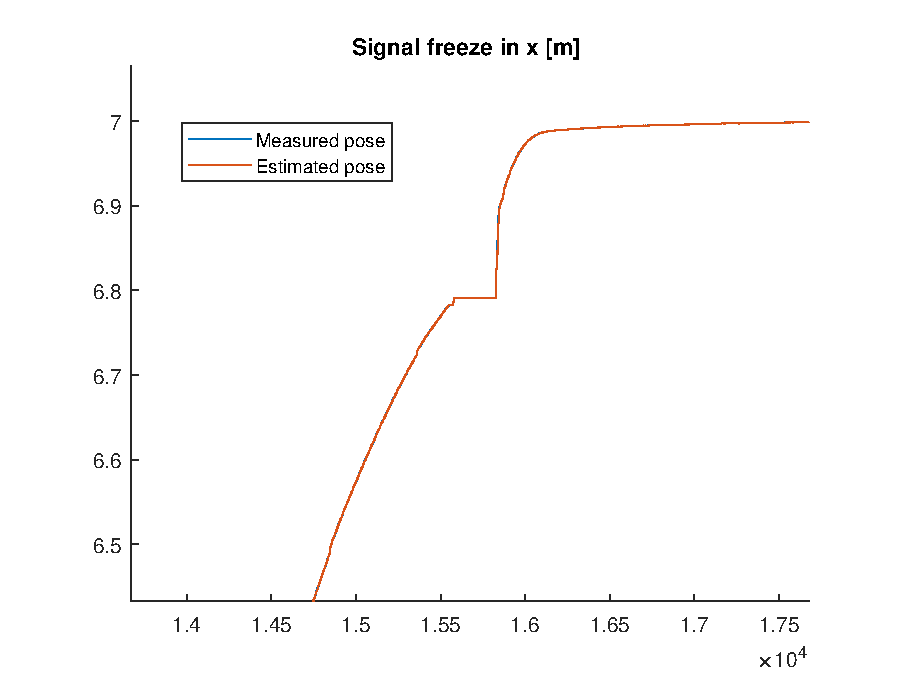
\includegraphics[width=0.9\textwidth]{plots/signal_freeze.eps}
\caption{"Frozen" measurement signal}
\label{fig:signal_freeze}
\end{figure}

In Fig. \ref{fig:signal_freeze}, as one can see, the pose measurement is still for around 250 samples, or 2,5 seconds, and while the control system assumes the ship is at a constant position, it is in the middle of a motion, and has a surge speed. When the camera system then again detects the ship, the pose is changed, and the estimate jumps to the new position, leading to a corresponding, sudden change in the velocity estimate, as seen in Fig. \ref{fig:surge_spike}. It is strongly desirable to avoid the velocity spikes, in addition to having a reliable estimate, to avoid false motions and thus noise in the control input. 

\begin{figure}[!h]
\centering
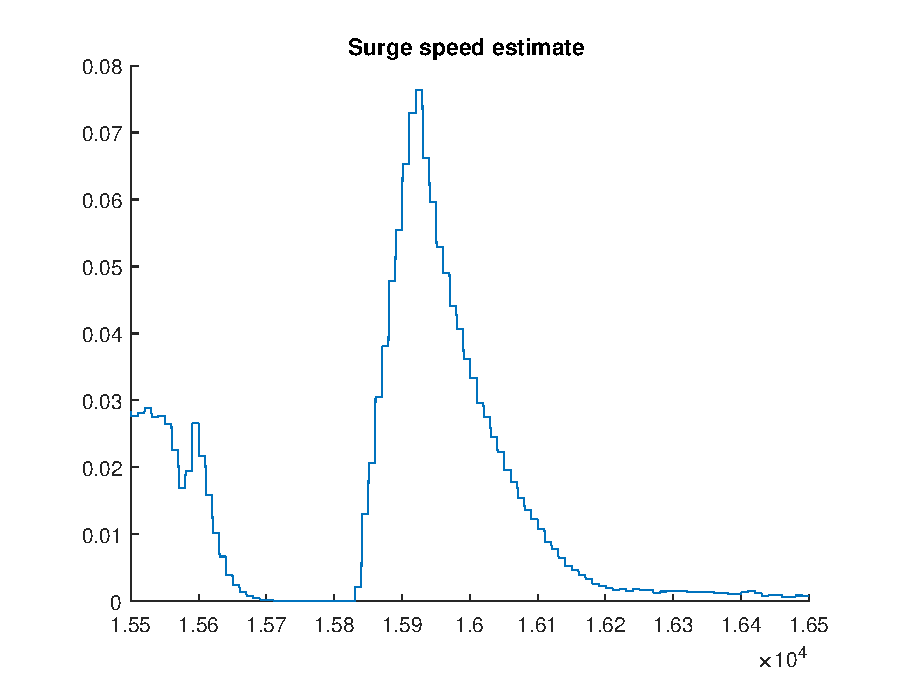
\includegraphics[width=0.9\textwidth]{plots/surge_spike.eps}
\caption{Sudden surge after recovering position measurement}
\label{fig:surge_spike}
\end{figure}

To ensure that the velocity estimator fault-tolerant to the phenomenons mentioned, and also more robust operation, a revision is proposed:\\ The estimator will have 3 states of operation; Normal operation, frozen measurement signal and rediscovered measurement signal. A subsystem is written in the control implementation, which compares each new sample to the previous down to the 8th decimal. The Qualisys system runs at 20Hz, while the control system runs at 100Hz, which means that every 5 consecutive samples from the camera system will be identical. If, however, the following sample is identical to the previous 5, at $10^8$ decimal precision in all DOF, the signal is assumed to have been lost. A Boolean "measurement frozen" signal is then sent to the estimator, which switches state. To avoid detecting false positives, the threshold for a lost signal is set to 7 consecutive identical measurement samples. 



The velocity estimator is written as a derivative filter using the pose measurements as input. For normal operation, this is implemented as such:
\begin{align}
    \boldsymbol{\eta}_{filtered(n)} &= a*\boldsymbol{\eta}_{measured(n)} + (1-a)*\boldsymbol{\eta}_{filtered(n-1)} \\
    \boldsymbol{\Dot{\eta}} &= \frac{\boldsymbol{\eta}_{filtered(n)}-\boldsymbol{\eta}_{filtered(n-1)}}{h} \\
    \boldsymbol{\Dot{\eta}}_{filtered(n)} &= b*\boldsymbol{\Dot{\eta}}_{measured} + (1-b)*\boldsymbol{\Dot{\eta}}_{filtered(n-1)}\\
    \boldsymbol{\hat{\nu}} &= \boldsymbol{R}^T(\psi)*\boldsymbol{\Dot{\eta}}_{filtered(n)},
\end{align}\label{eq:vel_estimator}
where h is the sample time in the control system, 0.01 second, and $a,b \in {\rm I\!R}$ are the cutoff-parameters for the filter. When the estimator detects a lost signal, it switches state and keeps the last recorded $\hat{\nu}$ to estimate the position until the camera system again detects the ship. While the signal is lost, the estimator will run as:

\begin{align}
    \boldsymbol{\hat{\eta}} &= \int \boldsymbol{R}(\hat{\psi})\boldsymbol{\hat{\nu}}\\
    \boldsymbol{\hat{\eta}}_{(0)} &= \boldsymbol{\hat{\eta}}_{(n-1)}
\end{align}

Then, when the measurement signal is recovered, it switches back to \ref{eq:vel_estimator}, and then initialized by:

\begin{align}
    \boldsymbol{\eta}_{filtered(n-1)} &= \boldsymbol{\hat{\eta}}_{(n-1)} \\
    \boldsymbol{\Dot{\eta}}_{filtered(n-1)} &= \boldsymbol{\hat{\nu}}_{(n-1)}
\end{align}
The block diagram for the re-written velocity estimator as implemented on CSAD can be seen in Fig. \ref{fig:estimator_blockdiagram}.

\begin{figure}
    \centering
    \begin{tikzpicture}
    \draw (-9,0.2) node[minimum height=1cm,minimum width=1cm,align=center,draw] (QTM) {QTM};
    \draw (-7,-1.5) node[minimum height=1cm,minimum width=1cm,align=center,draw] (SignalFrozen) {Signal\\ Observer};
    \draw (-4.5,0) node[minimum height=1.5cm,minimum width=1cm,align=center,draw] (DerivativeFilter) {Derivative\\Filter};
    \draw (-1.5,-1.3) node[minimum height=1cm,minimum width=1cm,align=center,draw] (LostNu) {Estimator\\Override};
    \draw (1,-1.1) node[minimum height=1cm,minimum width=1cm,align=center,draw] (Rotation) {$R(\psi)$};
    \draw (3,-1.1) node[minimum height=1cm,minimum width=1cm,align=center,draw] (Integrator) {$\frac{1}{s}$};
    \draw (2,0.2) node[minimum height=1cm,minimum width=1cm,align=center,draw] (Switch) {Switch};
    
    \draw[-latex] (QTM.east) |- ([xshift=1.4cm] QTM.east)  node[above]{$\eta$}|- ([yshift=0.2cm] DerivativeFilter.west);
    
    \draw[-latex] (QTM.east) -|([xshift=0.1cm] QTM.east) -|([xshift=-0.3cm] SignalFrozen.west) |-(SignalFrozen.west);
    
    \draw[-latex] (SignalFrozen.east) -| ([xshift=0.1cm] SignalFrozen.east) -|([xshift=-0.5cm,yshift=-0.3cm] DerivativeFilter.west) |-([yshift=-0.3cm] DerivativeFilter.west);
    
    \draw[-latex] (SignalFrozen.east) -| ([xshift=2cm] SignalFrozen.east) node[above]{signal\_lost} |- ([yshift=-0.2cm] LostNu.west);
    
    \draw[-latex] ([yshift=-0.4cm] DerivativeFilter.east)  -| ([xshift=0.5cm,yshift=-0.4cm] DerivativeFilter.east) node[above]{$\hat{\nu}$}  -| ([xshift=-0.25cm,yshift=0.2cm] LostNu.west) |- ([yshift=0.2cm] LostNu.west);
    
    \draw[-latex] (LostNu.east) |- ([yshift=-0.2cm] Rotation.west); 
    
    \draw[-latex] (QTM.east) -| ([xshift=0.415cm] QTM.east) -| ([xshift=0.415cm,yshift=1cm] QTM.east) -| ([xshift=-0.5cm,yshift=2.3cm] Rotation.west) -| ([xshift=-0.5cm,yshift=0.2cm] Rotation.west) |-([yshift=0.2cm] Rotation.west);
    
    \draw[-latex] (Rotation.east) -| ([xshift=0.45cm] Rotation.east) node[above]{$\dot{\hat{\eta}}$} |- (Integrator.west);
    
    \draw[-latex] (LostNu.east) -| ([xshift=0.5cm,yshift=-0.7cm] LostNu.east) -| ([xshift=1.2cm,yshift=-0.7cm] LostNu.east)  |- ([xshift=1.5cm,yshift=-0.7cm] LostNu.East) node[right]{$\hat{\nu}$};
    
    \draw[-latex] (Integrator.east) -| ([xshift=0.3cm] Integrator.east) node[above]{$\hat{\eta}$} -| ([xshift=0.6cm] Integrator.east) -| ([xshift=0.6cm,yshift=0.65cm] Integrator.east) -| ([xshift=-0.3cm,yshift=-0.55cm] Switch.west) -| ([xshift=-0.3cm,yshift=-0.2cm] Switch.west) |- ([yshift=-0.2cm] Switch.west);
    
    \draw[-latex] ([yshift=0.4cm] DerivativeFilter.east) -| ([yshift=0.4cm,xshift=0.5cm] DerivativeFilter.east) node[above]{$\hat{\eta}$} |- ([yshift=0.2cm] Switch.west);
    
    \draw[-latex] (Switch.east) |- ([xshift=1cm] Switch.east) node[right]{$\hat{\eta}$} 
    
    \end{tikzpicture}
    \caption{Block diagram for the updated velocity estimator}
    \label{fig:estimator_blockdiagram}
\end{figure}



\subsection{Ship model adjustment}

As discussed in Chapter 2.1.1, some adjustments to the ship model presented were needed from the model presented in \cite{bjorno} and \cite{bjørnø2017}. The first lab session is run with these parameter changes, see Table \ref{CSADParameters}. After the first lab session, behavior of the ship suggested that the model was not entirely accurate. 

\begin{table}[h!]
\centering 
\begin{tabular}{| p{2cm} | p{2cm} | p{3cm} | p{2cm}|}
\hline
\textbf{Parameter}& \textbf{Lab session 1 parameters } &  \textbf{Updated for session 2} &\textbf{Unit}   \\ \hline\hline
$L$ & $2.578$ & $2.578$ & $m$  \\ \hline
$m$ & $127.92$ &127.92 & $kg$ \\ \hline
$x_g$ & $0$ & $\boldsymbol{0.0375}$ & $m$  \\ \hline
$I_z$ & $62$& 62 & $kgm^2$  \\ \hline
$X_{\dot{u}}$ &$3.26$& $\boldsymbol{-3.26}$ & $kg $ \\ \hline
$Y_{\dot{v}}$ &$28.9$& $\boldsymbol{-28.9}$ & $kg$  \\ \hline
$Y_{\dot{r}}$ & $0.525$ & $\boldsymbol{-0.525}$ & $kgm$  \\ \hline
$N_{\dot{v}}$ &$0.157$ &$\boldsymbol{-0.157}$ & $kgm$ \\ \hline
$N_{\dot{r}}$ & $14$ &$\boldsymbol{-14}$ & $kgm^2$  \\ \hline
$X_u$ & $ -2.33$ &-2.33 &$kg/s$  \\ \hline
$X_{|u|u}$ & $0$ &0& $kg/m $ \\ \hline
$X_{uuu}$ & $-8.56$ & -8.56&$kgs/m^2$  \\ \hline
$Y_v$ & -4.67 &-4.67 &$kg/s$\\ \hline
$Y_{|v|v}$ & $0.398$ & $\boldsymbol{-0.398}$ & $kg/m$\\ \hline
$Y_{vvv}$ & $-313$ & -313& $kgs/m^2$\\ \hline
$N_v$ & $0$ & 0 &$kgm/s$\\ \hline
$N_{|v|v}$ & $-0.209$ &-0.209 & $kg/m$\\ \hline
$N_{vvv}$ & $0$&0 & $kgs/m^2$\\ \hline
$Y_r$ & $-7.25$ &-7.25 &$kgm/s$\\ \hline
$Y_{|r|r}$ & $-3.450$&-3.450 & $kg/m$\\ \hline
$Y_{rrr}$ & $0$&0 & $kgs/m^2$\\ \hline
$N_r$ & $-0.0168$ & $\boldsymbol{-7.141}$ &$kg/s$\\ \hline
$N_{|r|r}$ & $-0.0115$&$ \boldsymbol{-4.888} $& $kgm^2$\\ \hline
$N_{rrr}$ & $-0.000358$&$\boldsymbol{-0.152}$ & $kgs/m^2$\\ \hline
$N_{|v|r}$ & $0.08$&0.08 & $kg/m$\\ \hline
$N_{|r|v}$ & $0.08$& 0.08& $kg/m$\\ \hline
$Y_{|v|r}$ & $-0.845$ &-0.845 &$kg$\\ \hline
$Y_{|r|v}$ & $-0.805$ & -0.805&$kg$\\ \hline
\end{tabular}
\caption{Numerical values of the ship model parameters for CSAD.}
\label{CSADParameters}
\end{table}


\newpage
\subsection{Parameter gain adjustment}

\subsubsection{$\mathcal{L}_1$ adaptive control}

Before the first lab session, the parameter gains for the controller was tuned with simulations. In the real conditions in the lab basin however, it became clear that some adjustments were needed. Among these, it is worth mentioning the updating the gains for the state predictor. The L2 gain should be of greater magnitude than the L1 gain, a relation not maintained in lab session 1, see Table \ref{table:gains1}. The predictor L2 parameter is increased by a factor of 3, to ensure this relation. After the re-written velocity estimator is implemented, a double 4-corner test is performed for the $\mathcal{L}_1$ controller, one with the previous value, and one updated. 

\begin{figure}[h!]
\centering
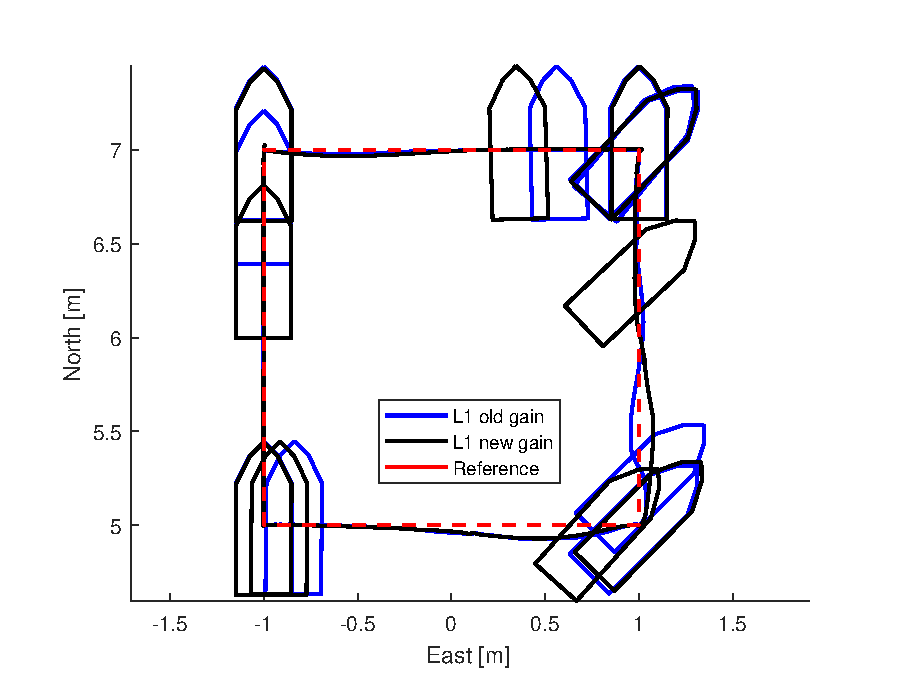
\includegraphics[width=0.9\textwidth]{adjustment_plots/4cornerimprovement.eps}
\caption{4-corner test comparing predictor gain adjustment}
\label{fig:4corner_newL2}
\end{figure}




\begin{table}[h!]
\centering
\caption{Performance metric comparison - Updated L2 gain}\label{table:comparingL2gaintable}
\begin{tabular}{lllll}
\cline{1-4}
\multicolumn{1}{|l|}{\textbf{L2 gain value}} & \multicolumn{1}{l|}{\textbf{IAE}} & \multicolumn{1}{l|}{\textbf{IAEW}} & \multicolumn{1}{l|}{\textbf{IADC}} &  \\ \cline{1-4}
\multicolumn{1}{|l|}{I*2*1.2*2*\pi} & \multicolumn{1}{l|}{76} & \multicolumn{1}{l|}{1231} & \multicolumn{1}{l|}{253} &  \\ \cline{1-4}
\multicolumn{1}{|l|}{I*2*1.2*2*\pi*3} & \multicolumn{1}{l|}{77} & \multicolumn{1}{l|}{722} & \multicolumn{1}{l|}{155} &  \\ \cline{1-4}
 &  &  &  & 
\end{tabular}
\end{table}

As seen in Fig. \ref{fig:4corner_newL2} and \ref{fig:metric_newL2}, there is not really a significant difference in overall pose error for the 4-corner test. However, the updated predictor gain greatly reduces the power consumption by the IAEW metric, and the actuator wear. This can be seen by Fig. \ref{fig:metric_newL2} and in Table \ref{table:comparingL2gaintableb}, where the final values of the metrics are displayed. The IAEW metric is reduced by $41\%$ and the IADC by $38\%$, which is a substantial decrease. This parameter change will be kept into the second lab session.

\begin{figure}[h!]
\centering
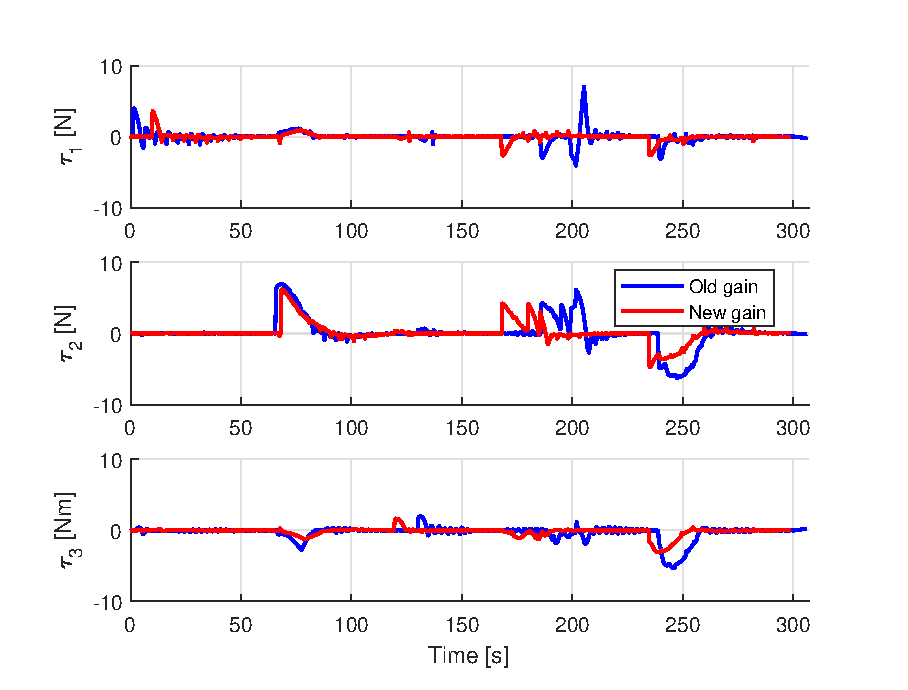
\includegraphics[width=0.9\textwidth]{adjustment_plots/tauimprovement.eps}
\caption{Control inputs comparing predictor gain adjustment}
\label{fig:tau_newL2}
\end{figure}

Fig. \ref{fig:tau_newL2} shows the time evolution of the control input. The overall lower amplitude gives reduced power consumption, but does not lead to a longer run-time of the 4-corner test.

\begin{figure}[!h]
\centering
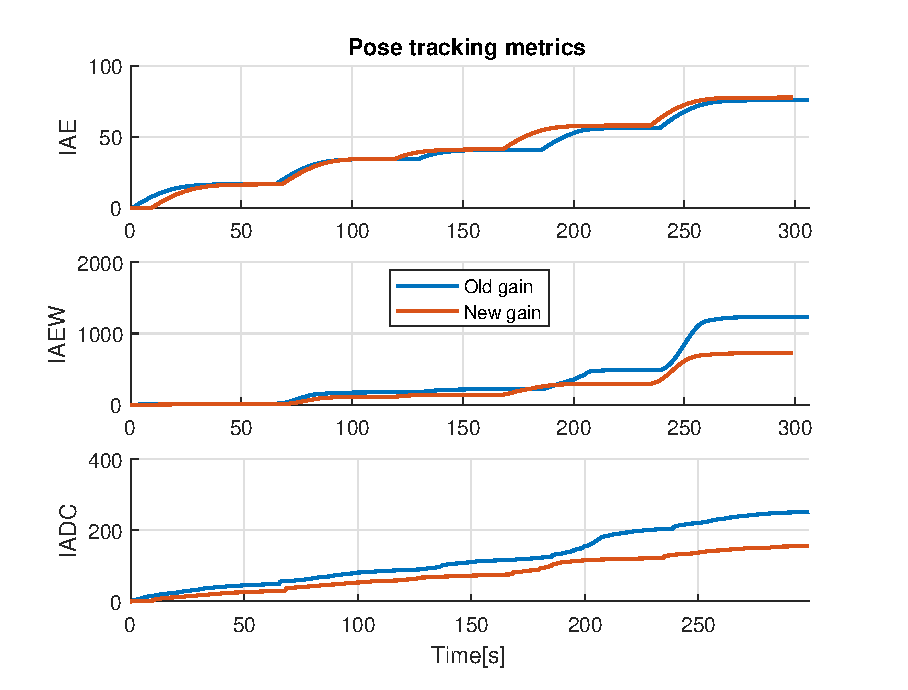
\includegraphics[width=0.9\textwidth]{adjustment_plots/metricimprovement.eps}
\caption{Performance metrics for comparing predictor gain adjustment}
\label{fig:metric_newL2}
\end{figure}




\newpage
\newpage
\section{Lab session 2 - May}

As in the first lab session, a non-adaptive NP-NV cascaded feedback controller will be used as a nominal base for comparison and to evaluate the performance of the adaptive scheme in this session. The NP-NV test is done under the new conditions as described in the previous section. The 4-corner test for the NP-NV is shown in Fig.  \ref{NPNV4corner2}. It can be observed that the adjustments of both velocity estimator and model parameters has an improving effect on the nominal NP-NV controller, especially for the ($4 \xrightarrow{} 4$) movement. The pose error IAE metric for NP-NV is also reduced by 14\%, from 92 to 79. 

\begin{figure}[!h]
    \centering
    \makebox[\textwidth][c]{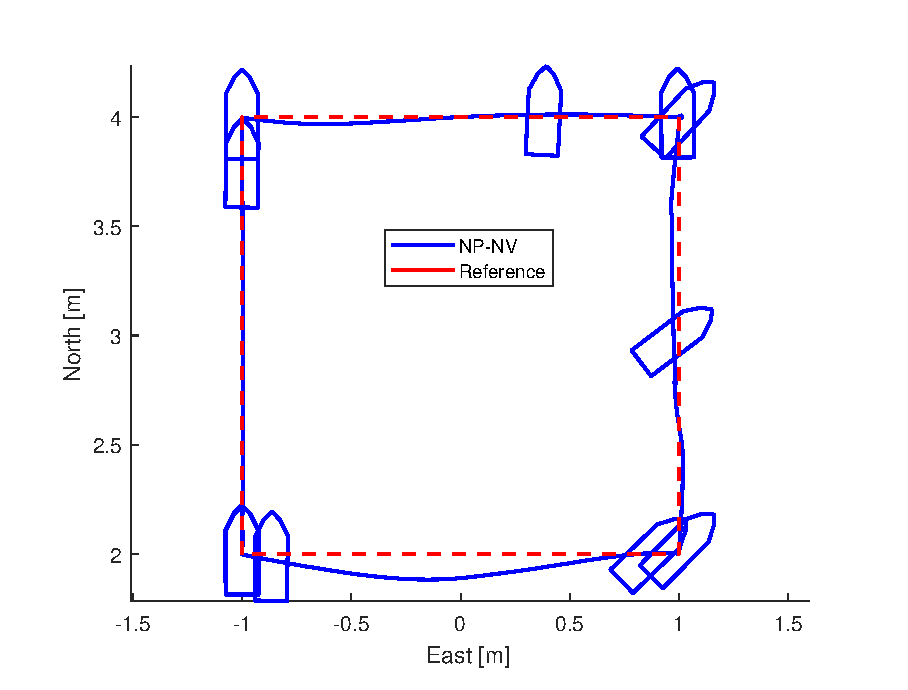
\includegraphics[width=0.7\textwidth]{lab2plots/NPNVpath.eps}}
    \caption{Unconstrained NPNV 4-corner test }
\end{figure}\label{NPNV4corner2}


The change of the North-axis of the 4-corner surface plots in this session, from (5-7) to (2-4), is due to a full re-calibration of the camera system, with the goal of reducing inaccuracies in the measurements. Besides from that, the 4-corner experiments are performed in the same fashion as the first session. 





\begin{table}[h!]
\centering
\caption{Control gains}\label{table:gains1}
\begin{tabular}{|l |c|r|}
\toprule
& \textbf{$\mathcal{L}_1$}  \\
\midrule
\hline
$\boldsymbol{\Gamma}_1$ & $\text{diag}([0.08,0.08,0.0698])$  \\

$\boldsymbol{\Gamma}_2$  & $\text{diag}([0.2,0.2,0.1745])\boldsymbol{M}$   \\

$\Delta_{\tilde{p}}$  & $0.5$    \\
$\Delta_{\tilde{\psi}}$  & $0.5$    \\

$\Delta_{\tilde{v}}$  & $0.7$ \\
$\Delta_{\tilde{r}}$  & $1$ \\
$\boldsymbol{L_1}$  & $I*(2*\pi)^2$ \\
$\boldsymbol{L_2}$  & $I*2*1.2*2*\pi*3$ \\
$\boldsymbol{\gamma}_w_{\delta}$  & $(20*\pi)^2/4$ \\\hline
\bottomrule

\end{tabular}
\end{table}
Table \ref{table:gains1} displays the control and parameter gains used for the second lab session. 

\subsection{$\mathcal{L}_1$ Adaptive control}

\begin{align}
    \boldsymbol{\tau} &= \boldsymbol{M}\dot{\alpha} + (\boldsymbol{C + D})\alpha - \boldsymbol{K}_2\boldsymbol{z}_2 -\boldsymbol{\hat{w_{\delta}}}  \\
    \boldsymbol{\dot{\hat{w_{\delta}}}} &=-\gamma_{w_\delta}\tilde{\boldsymbol{\nu}} 
\end{align}

\begin{figure}[!h]
    \centering
    \makebox[\textwidth][c]{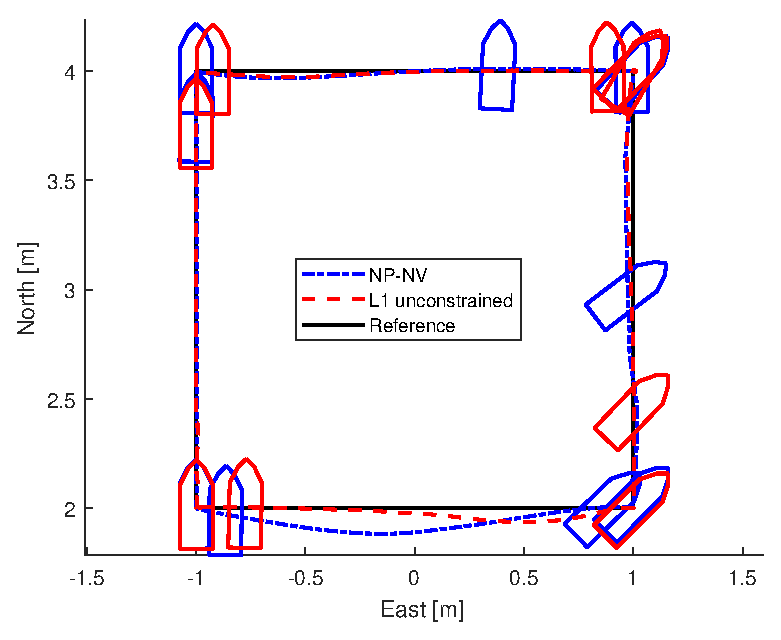
\includegraphics[width=0.7\textwidth]{lab2plots/L1path.eps}}
    \caption{Unconstrained $\mathcal{L}_1$ 4-corner test. }
\end{figure}\label{fig:L14corner2}

Fig. shows the surface plot of the unconstrained $\mathcal{L}_1$. It can be seen that the reference tracking has been improved from the previous session, and the $\mathcal{L}_1$ has improved tracking over the nominal controller, in particular for the  ($5 \xrightarrow{} 1$) motion. 

\begin{figure}[!h]
    \centering
    \makebox[\textwidth][c]{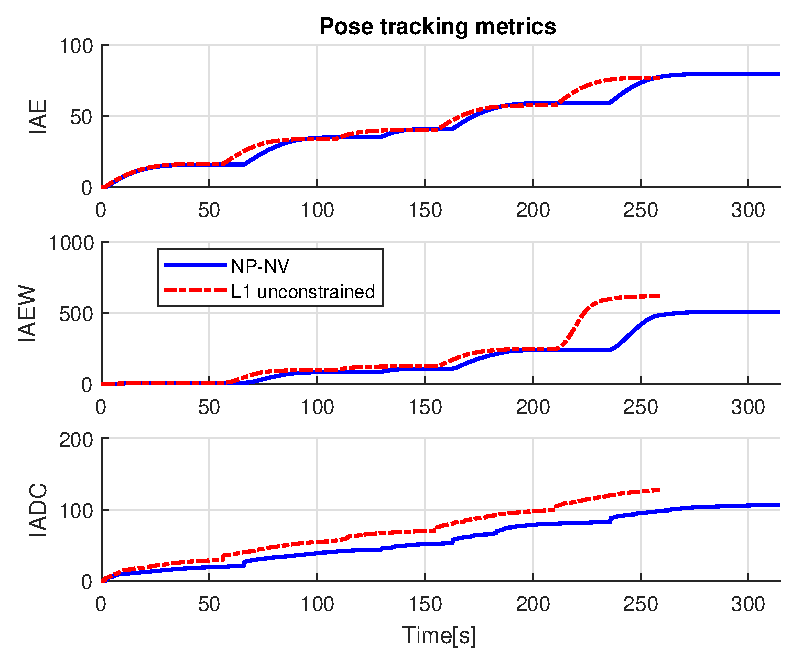
\includegraphics[width=0.7\textwidth]{lab2plots/L1metric.eps}}
    \caption{Unconstrained $\mathcal{L}_1$, Pose error metrics. }
\end{figure}\label{fig:L1metric2}

In Fig. \ref{fig:L1metric2} the time evolution of the performance metrics is shown. The unconstrained $\mathcal{L}_1$, as in the first session, is overall faster and more accurate in reference tracking than the NP-NV for the 4-corner test. Note that even though the adaptive control is higher in terms of energy consumption IAEW and wear IADC, the difference from the nominal is significantly reduced from the first lab session. This improvement is likely due to the improved velocity estimation, as well as the upscaled L2 gain which was discussed in the last section. As a result, the adaptation is less exposed to measurement noise and this leads to a cleaner control input signal, which can be seen in Fig. \ref{fig:L14tau2}.

\begin{figure}[!h]
    \centering
    \makebox[\textwidth][c]{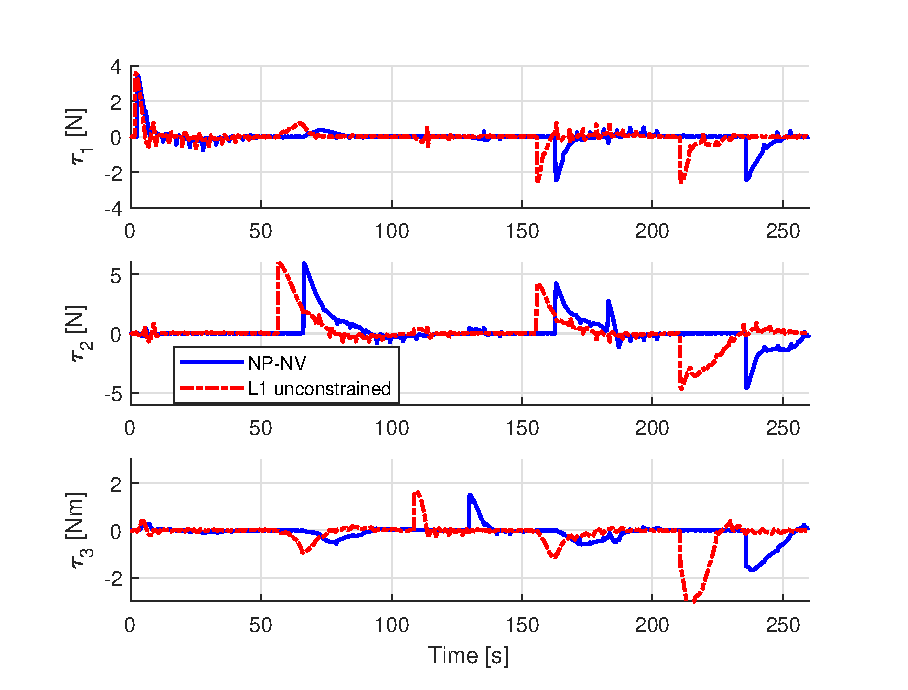
\includegraphics[width=0.7\textwidth]{lab2plots/L1tau.eps}}
    \caption{Unconstrained $\mathcal{L}_1$, Control input }
\end{figure}\label{fig:L14tau2}


\begin{figure}[!h]
    \centering
    \makebox[\textwidth][c]{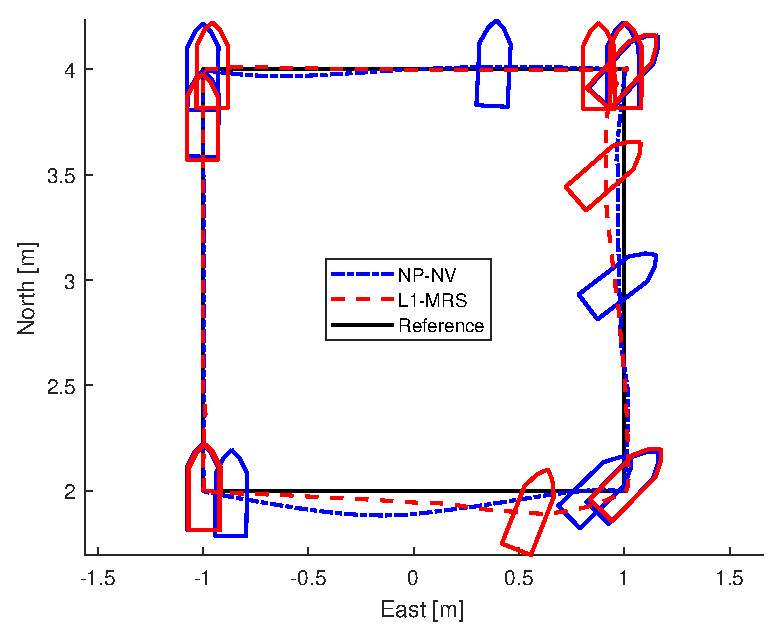
\includegraphics[width=0.7\textwidth]{lab2plots/L1MRS1path.eps}}
    \caption{$\mathcal{L}_1$ with MRS 4-corner test. Magnitude limits as in Table \ref{table} }
\end{figure}\label{fig:L1MRS4corner2}

As mentioned in the discussion from the first lab session, the cascaded $\mathcal{L}_1$-MRS control yielded promising results. The MRS model limitations are tuned according to a more realistic behavior on the basis of tests done on the ship actuator setup, as mentioned in the previous section, see Table \ref{table} The path plot of the first MRS test is shown in Fig. \ref{fig:L1MRS4corner2}. 

It can be observed that the adaptive follows the path good, although with some slip during the last 2 motions. This indicates that the magnitude limits could be too conservative for the $\mathcal{L}_1$. Even though that the ship is not physically able to output the desired force from $\mathcal{L}_1$, it could be that the high-gain adaptation gives a more suited control input than the set limitations of the MRS. 

\begin{figure}[!h]
    \centering
    \makebox[\textwidth][c]{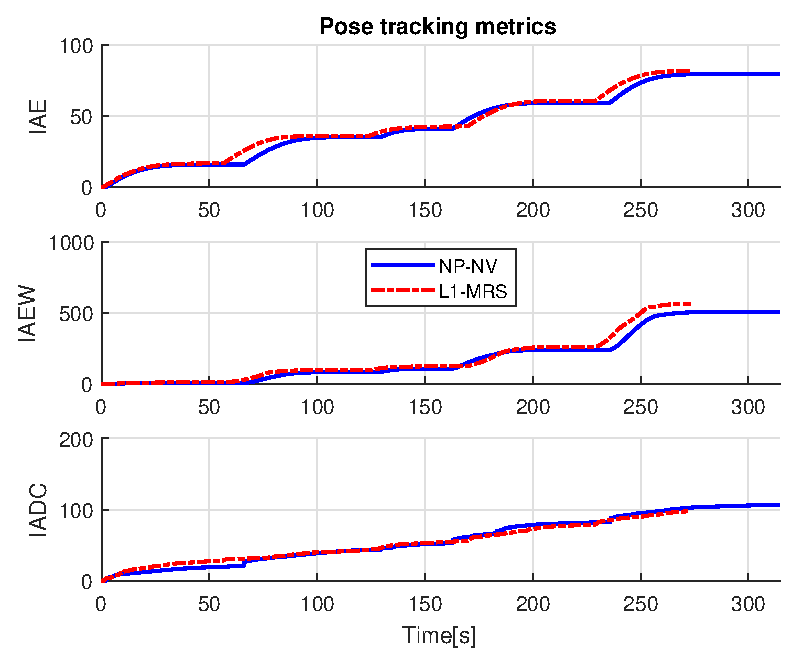
\includegraphics[width=0.7\textwidth]{lab2plots/L1MRS1metric.eps}}
    \caption{$\mathcal{L}_1$ with MRS, Pose error metrics. Magnitude limits as in Table \ref{table} }
\end{figure}\label{fig:L1MRSmetric2}

The pose error metrics for $\mathcal{L}_1$-MRS are shown in Fig. \ref{fig:L1MRSmetric2}. Note that the adaptive controller has reduced control rate metric IADC, or wear, than the nominal NP-NV. 
\begin{figure}[!h]
    \centering
    \makebox[\textwidth][c]{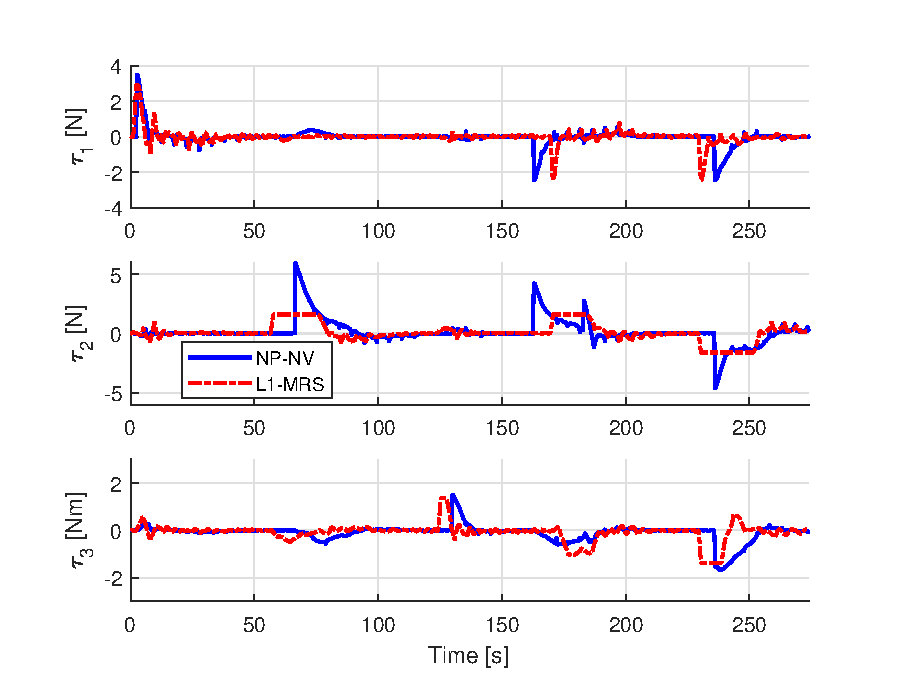
\includegraphics[width=0.7\textwidth]{lab2plots/L1MRS1tau.eps}}
    \caption{$\mathcal{L}_1$ with MRS, Control input. Magnitude limits as in Table \ref{table}.}
\end{figure}\label{fig:L1MRS4tau2}

\begin{figure}[!h]
    \centering
    \makebox[\textwidth][c]{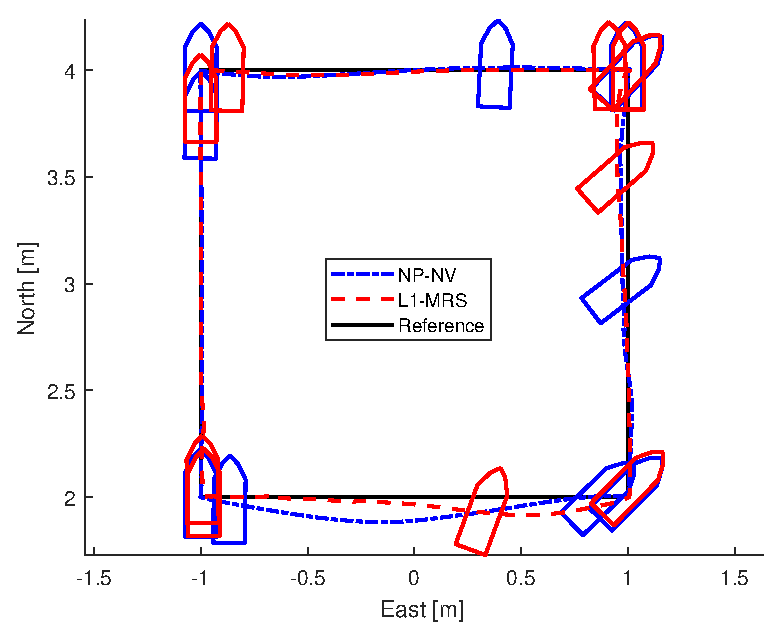
\includegraphics[width=0.7\textwidth]{lab2plots/L1MRS2path.eps}}
    \caption{$\mathcal{L}_1$ with MRS 4-corner test. Magnitude limit [5 5 3]$^\top{}$.}
\end{figure}\label{fig:L1MRS24corner2}

As it the last $\mathcal{L}_1$-MRS experiment could indicate that the magnitude saturation limits were too conservative, the limits are then set to [5 5 3]$^\top{}$ with the goal of improving tracking by higher thrust allowance at the cost of energy consumption. The path plot is shown in Fig. \ref{fig:L1MRS24corner2}. As can be seen, the boat achieves better track following than in the last experiment, as well as NP-NV. 

\begin{figure}[!h]
    \centering
    \makebox[\textwidth][c]{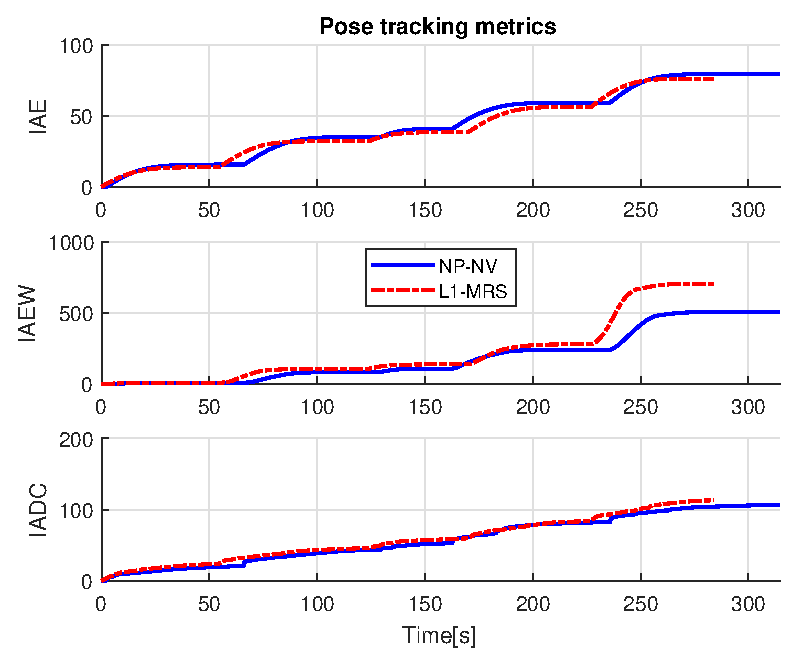
\includegraphics[width=0.7\textwidth]{lab2plots/L1MRS2metric.eps}}
    \caption{$\mathcal{L}_1$ with MRS, Pose error metrics. Magnitude limit [5 5 3]$^\top{}$.}
\end{figure}\label{fig:L1MRS2metric2}

However, as assumed the higher allowance increases energy consumption IAEW by 22 percent compared to the conservative magnitude limits, as can be seen in Table \ref{performancemetrics2} and the metric plot in Fig. \ref{fig:L1MRS2metric2}. Fortunately, the IADC is similar to the nominal, indicating that the rate limits of the MRS has a positive effect on the $\mathcal{L}_1$ adaptation.

\begin{figure}[!h]
    \centering
    \makebox[\textwidth][c]{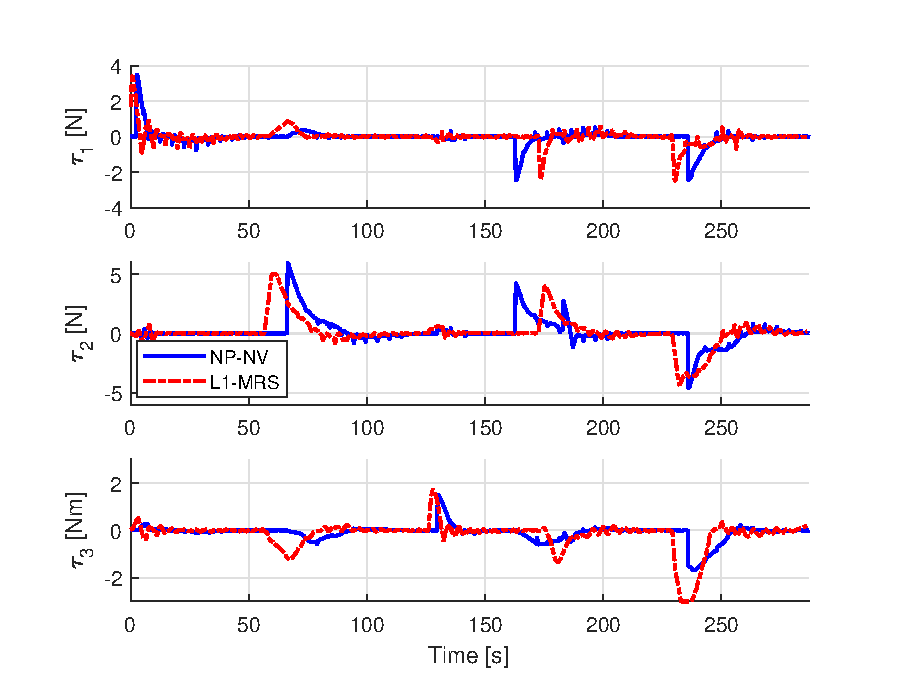
\includegraphics[width=0.7\textwidth]{lab2plots/L1MRS2tau.eps}}
    \caption{$\mathcal{L}_1$ with MRS, Control input. Magnitude limit [5 5 3]$^\top{}$.}
\end{figure}\label{fig:L1MRS24tau2}

\newpage

\subsection{Summary of lab session 2}
It is a known behavior for all controllers to slip in North-coordinate during the final motion ($5 \xrightarrow{} 1$) coupled motion displayed in Fig. \ref{fig:4corner}. A notable similarity seen in the $\mathcal{L}_1$ experiments, is that adaptive controller corrects for this error fast, whereas the nominal NP-NV first reduces control error in heading before correcting surge. This is likely due to how the adaptation weights the errors in each DOF. 

\begin{table}[h!]
\centering 
\begin{tabular}{| p{2cm} | p{2cm} | p{3cm} | p{2cm}|}
\hline
\textbf{Controller}& \textbf{IAE} &  \textbf{IAEW} &\textbf{IADC}   \\ \hline\hline
$NP-NV$ & $79$ & $505$ & $107$  \\ \hline
$\mathcal{L}_1 unconstr.$ & $76$ & $614$ & $127$  \\ \hline
$\mathcal{L}_1 MRS$ & $81$ & $562$ & $97$  \\ \hline
$\mathcal{L}_1 MRS-high$ & $78$ & $729$ & $115$  \\ \hline

\end{tabular}
\caption{End values of performance metrics - pose error}
\label{performancemetrics2}
\end{table}
Table \ref{performancemetrics1} lists the final maximum values for the tested control implementations in lab session 2. The metric values are rounded to the nearest integer for readability.


\section{Discussion}

\cleardoublepage